% \documentclass[twocolumn]{article}
\documentclass{article}
% \documentclass[useAMS,usenatbib]{mnras}
\usepackage[utf8]{inputenc}

\usepackage{graphicx}% Include figure files
\usepackage{xcolor}
\usepackage{epstopdf}% Allows eps figures
\usepackage{float}% Better image placement
\usepackage{enumerate}

\usepackage{textcomp,gensymb}% Adds general symbols
\usepackage{amsmath, amssymb}% Math symbols and stuff
\usepackage{mathtools}% math things

\usepackage[numbers,sort&compress]{natbib}% Hyperlink References
\usepackage{hyperref}% Hyperlink References

\usepackage{ulem}
\usepackage[capitalise]{cleveref}

\newcommand{\dnp}[1]{\textcolor{cyan}{#1}}


\title{Quick Notes about Machine Learning on Intensity Maps}
\author{Daniel N. Pfeffer}
\date{}

\graphicspath{{images/}}

\begin{document}
% \bibliographystyle{unsrtnat}

	\maketitle

	\begin{abstract}
		The idea of this project is to use machine learning on intensity maps to determine the luminosity function of the underlying halos.
	\end{abstract}

	\section{Jump to Section}
		\begin{enumerate}
			\item IM backgroundish \ref{sec:IMback}

			\item ML background \ref{sec:MLback}

			\item First CNN work \ref{sec:cnn}

			\item Second batch of CNN work \ref{sec:cnn2}

			\item Third wave of CNN work \ref{sec:arch}

			\item Third wave with noise \ref{sec:noise}

			\item Compare to Power Spectrum Method \ref{sec:power_compare}

			\item Accidentally Memorizing \ref{sec:mem}

			\item Using Random Parameters in Models \ref{sec:rand}

			\item Comparing Multiple Models \ref{sec:mult}

			\item Memorization Realization \ref{sec:ohcrap}

			\item Something Finally Works \ref{sec:works}

			\item To do list \ref{sec:todo}
		\end{enumerate}	

	\section{Intensity Maps Background} \label{sec:IMback}

		Intensity mapping is done by looking at a given emission line.  Whatever is being traced should be emitting this line at any location where the tracer is located.  Having a higher density of the tracer would cause an increased intensity of whatever line is being looked at.  As the light travels to Earth it will get redshifted based on where it was originally emitted.  By looking at a range of frequencies one can get 3D spatial information (maps) about whatever tracer is being looked at.  

		George has code to generate different halo catalogs quickly and has done so to make (as of the time of writing this part) 161 halo catalogs.  Each of these catalogs can be converted into smaller subfields as well as rotated to produce more catalogs.  With another code of George's one can convert these halo catalogs (or regions in them) into intensity maps.  We want lots of intensity maps so that we can do machine learning on the maps to determine the underlying luminosity function.

	\section{Machine Learning Background} \label{sec:MLback}

		I'm feeling lazy right now and don't want to fully flesh this out yet.

		Machine learning can be used for lots of tings if you throw enough data at it.  

		Neural networks are supposed to represent how brains and neurons work.  It is trained for a specific task and each neuron has it's own weights.  This gets very memory intensive for large networks because there can be lots of neurons.  A way around this is to use convolutional neural networks (CNN).  A CNN has filters that convolve with layers of input or neuron output and each layer has the same filter which saves on memory.  A quick Google showed these links that explain CNNs both in depth (http://cs231n.github.io/convolutional-networks/) and at a surface level (https://medium.freecodecamp.org/an-intuitive-guide-to-convolutional-neural-networks-260c2de0a050).

	\section{Intensity Mapping CNN (Actually on N not dN/dL)} \label{sec:cnn}

		As of right now the idea is to use a CNN on simulated intensity maps to determine the luminosity function of the underlying halos that made the simulated intensity maps.  George has code to make the halo catalogs and another code to convert the catalogs into intensity maps.  I've made code to split up the catalogs into smaller subfields to match possible experiments.  I also have code that will rotate the halo catalogs before making subfields so that we have more subfields to train out network with.  George's code limlam mocker (llm) (the code that converts catalogs into intensity maps) was modified by me to also give out the luminosity function of the underlying halos.  The llm can also use different underlying halo luminosity relations to generate different maps and luminosity functions.

		As of the basic training right now I am not doing anything to split up the maps into training, validation and test sets.  I'm just seeing the general results of different things right now.

		\subsection{log dN/dL} \label{sec:logValue}
			Originally the CNN was trained on converting an intensity map into \(\log dN/dL\) instead of just \(dN/dL\).  This was done originally to prevent having such a large range of output values could be hard to train.

			As of right now I have a trained network that is 4 layers that trained for 100 epochs of 400 maps apiece.  Each layer is a 3D convolution with kernel size 5 and stride 1 followed by a max pooling 3D of size 2 and stride 2.  The first layer has 32 filters, followed by 64, 128 and 256.  Following the convolutional layers the network is flattened and then has a dense layer with 1000 neurons.  The final layer is another dense layer with a neuron for each point in the luminosity function we want.  Currently I take 50 points of the luminosity function.  The loss function was just the mean square error function.

			\dnp{Should get plots for accuracy and loss as a function of time, but forgot to add that functionality to the CNN when I first ran it}.  The network took under 30 hours to train.  \cref{fig:CNN_4_layer_log,fig:CNN_4_layer_log_ratio,fig:CNN_4_layer_log_ratio_small} show the result of the CNN on some random map.  In all luminosity bins before around \(L = 10^6 L_{sun}\) the CNN luminosity function is within a couple of percent of the underlying one.  After \(L = 10^6 L_{sun}\) the ratio of CNN luminosity function to the given luminosity function jumps up to around 1.6.  The specific values change depending on what map is used, but they all show the issue at large luminosities.

			\begin{figure}[H]
				\centering 
				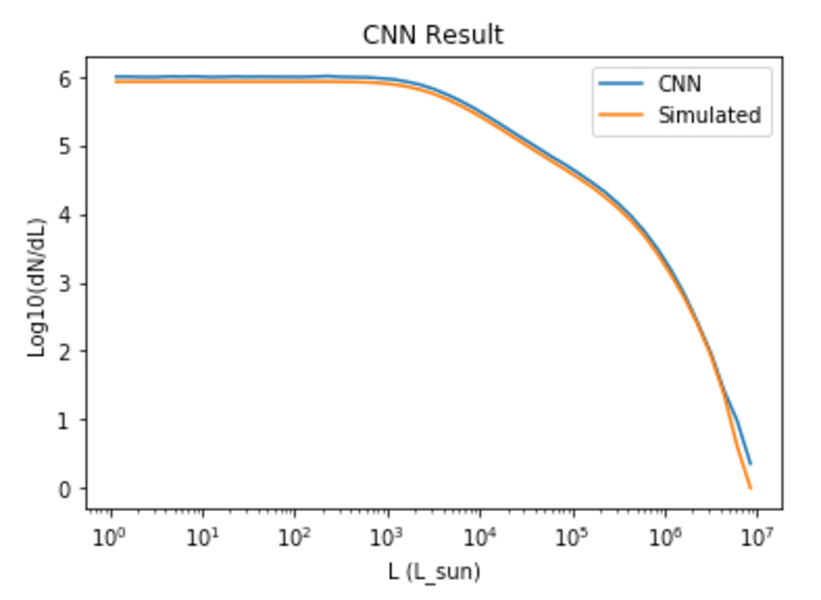
\includegraphics[width=0.8\textwidth]{CNN_4_layer_log.pdf}
				\caption{Plot showing the comparison of the output of the 4 layer CNN to the expected result of the underlying luminosity function that made the intensity map.}
				\label{fig:CNN_4_layer_log}
			\end{figure}

			\begin{figure}[H]
				\centering
				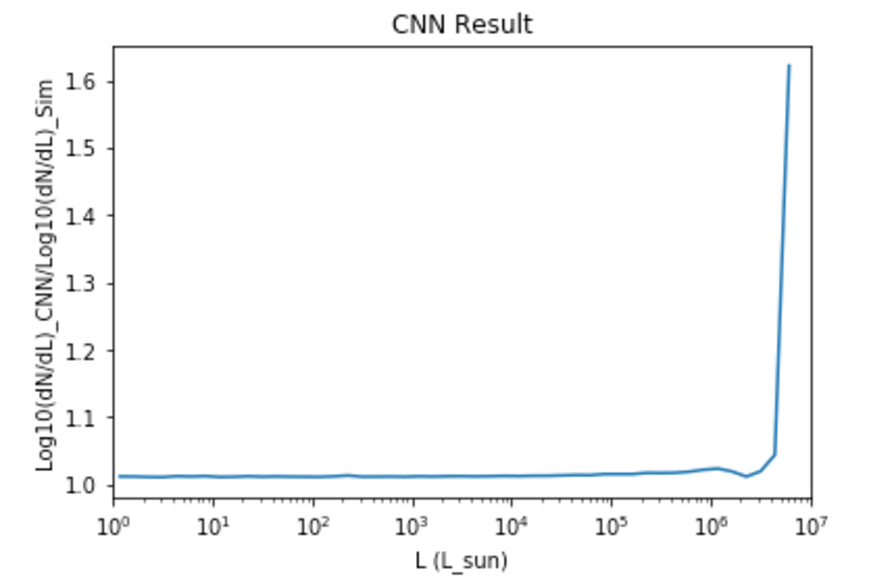
\includegraphics[width=0.8\textwidth]{CNN_4_layer_log_ratio.pdf}
				\caption{Plot showing the ratio of the CNN luminosity function over the underlying luminosity function.}
				\label{fig:CNN_4_layer_log_ratio}
			\end{figure}

			\begin{figure}[H]
				\centering
				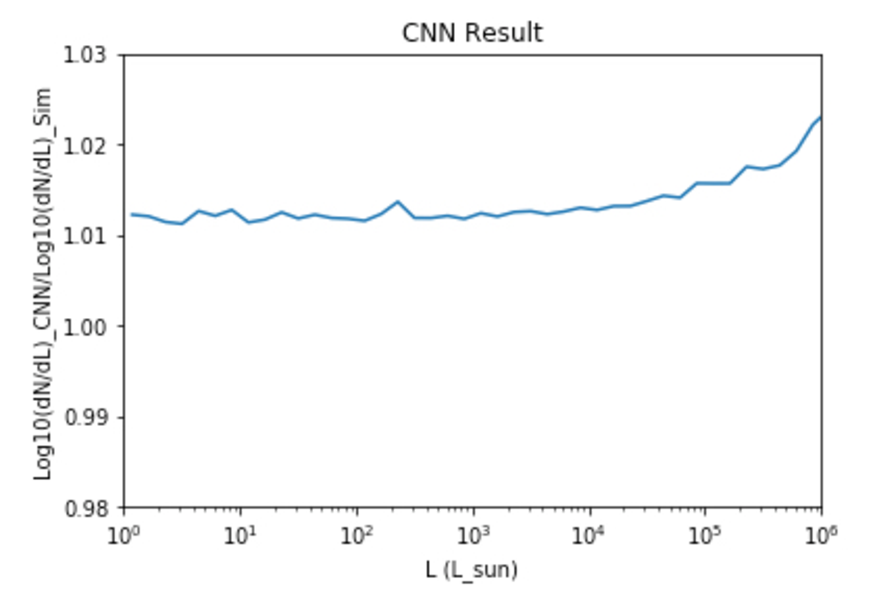
\includegraphics[width=0.8\textwidth]{CNN_4_layer_log_ratio_small.pdf}
				\caption{Zoom in of Figure \ref{fig:CNN_4_layer_log_ratio} showing the ratio of values before \(L = 10^6 L_{sun}\).}
				\label{fig:CNN_4_layer_log_ratio_small}
			\end{figure}

			We are probably interested in the actual values of things and not the log value so I checked the accuracy of the values instead of the log values.  The same set of plots but without logs are shown in \cref{fig:CNN_4_layer_log_unlog,fig:CNN_4_layer_log_unlog_ratio,fig:CNN_4_layer_log_unlog_ratio_small}.  What can be seen is that the error increases by at least an order of magnitude.  The error is still only around 20\%, but is still much larger then in the log case.  It can be shown (but I'm too lazy to type it out now) that the ratio of the unloged values is actually given by
			\begin{equation}
				\frac{dN}{dL}_{\rm{CNN}} / \frac{dN}{dL}_{\rm{sim}}(L) = 10^{\log \left(\frac{dN}{dL}_{\rm{sim}} (L)\right) * y(L)}
			\end{equation}
			where 
			\begin{equation}
				y = \log \left( \frac{dN}{dL}_{\rm{CNN}} \right) / \log \left( \frac{dN}{dL}_{\rm{sim}} \right)(L).
			\end{equation}

			\begin{figure}[H]
				\centering
				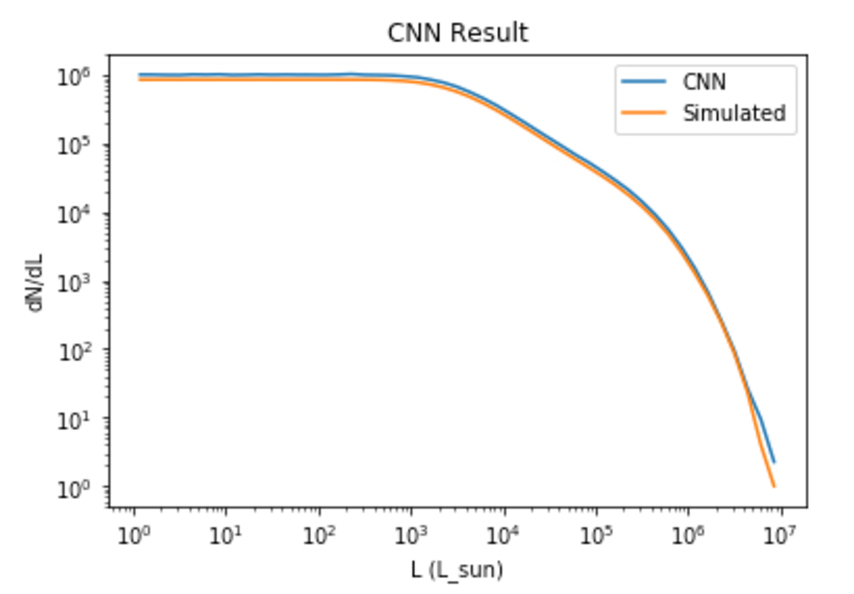
\includegraphics[width=0.8\textwidth]{CNN_4_layer_log_unlog.pdf}
				\caption{Plot showing the comparison of the output of the 4 layer CNN to the expected result of the underlying luminosity function that made the intensity map.}
				\label{fig:CNN_4_layer_log_unlog}
			\end{figure}

			\begin{figure}[H]
				\centering
				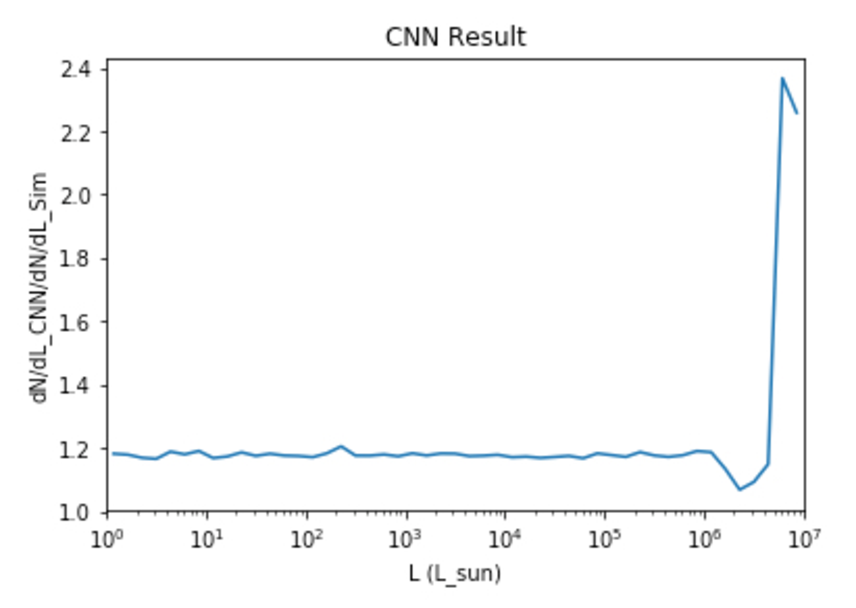
\includegraphics[width=0.8\textwidth]{CNN_4_layer_log_unlog_ratio.pdf}
				\caption{Plot showing the ratio of the CNN luminosity function over the underlying luminosity function.}
				\label{fig:CNN_4_layer_log_unlog_ratio}
			\end{figure}

			\begin{figure}[H]
				\centering
				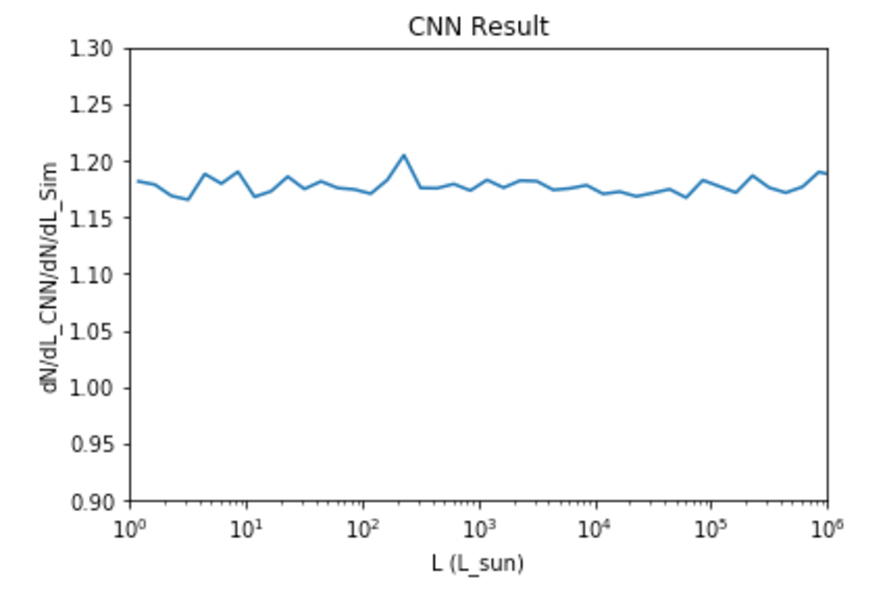
\includegraphics[width=0.8\textwidth]{CNN_4_layer_log_unlog_ratio_small.pdf}
				\caption{Zoom in of Figure \ref{fig:CNN_4_layer_log_ratio} showing the ratio of values before \(L = 10^6 L_{sun}\).}
				\label{fig:CNN_4_layer_log_unlog_ratio_small}
			\end{figure}

		\subsection{4 Layer dN/dL} \label{sec:4directValue}
			Seeing that finding the log luminosity value gives errors around 20\%, I tried to see if we could find the actual luminosity function directly.  The first network was 4 layers and was trained for 100 epochs of 400 maps apiece.  Each layer is a 3D convolution with kernel size 5 and stride 1 followed by a max pooling 3D of size 2 and stride 2.  The first layer has 32 filters, followed by 64, 128, 256 512.  Following the convolutional layers the network is flattened and then has a dense layer with 1000 neurons.  The final layer is another dense layer with a neuron for each point in the luminosity function we want.  Currently I take 50 points of the luminosity function.  The loss function was the mean log square error function.  Using mlse instead of mse makes it so that it doesn't get stuck trying to fit the region of low L and ignore the higher L regions where dN/dL is smaller. 

			I forget how long the network took to train, but it was under 48 hours.  Looking at \cref{fig:CNN_4_layer,fig:CNN_4_layer_ratio} one can see that the training did not go as well as it could.  There are discontinuities in the outputted luminosity function, sharp spikes and nothing after \(L \approx 10^6 L_{\rm{sun}}\).  I'm no expert, but we would want something better then that.  \cref{fig:CNN_4_layer_history_mlse,fig:CNN_4_layer_history_mse} show the training history of the loss function and another metric as a function of epoch while training 4 layer network.  The shape of \cref{fig:CNN_4_layer_history_mse} does look like what one would expect from a loss function.

			\begin{figure}[H]
				\centering
				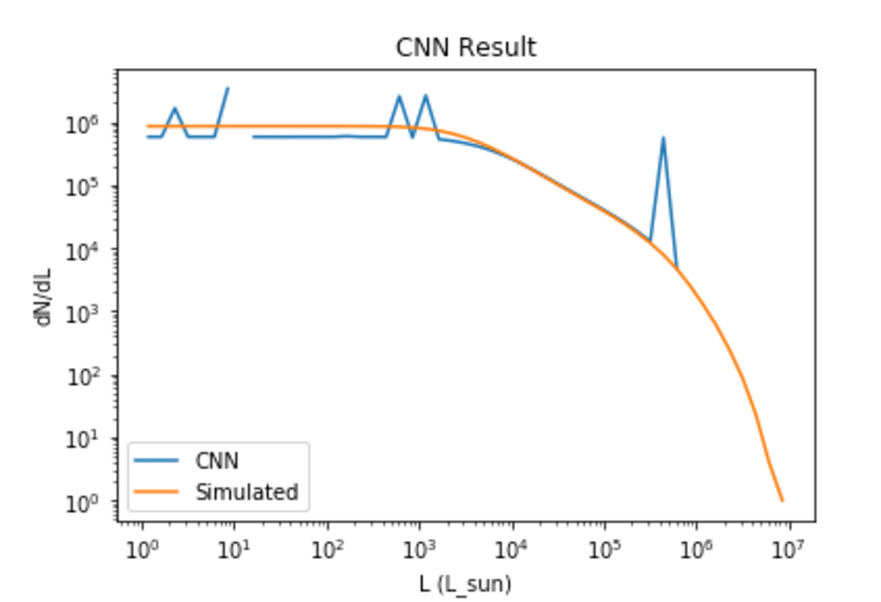
\includegraphics[width=0.8\textwidth]{CNN_4_layer.pdf}
				\caption{Plot showing the comparison of the output of the 4 layer CNN to the expected result of the underlying luminosity function that made the intensity map.}
				\label{fig:CNN_4_layer}
			\end{figure}

			\begin{figure}[H]
				\centering
				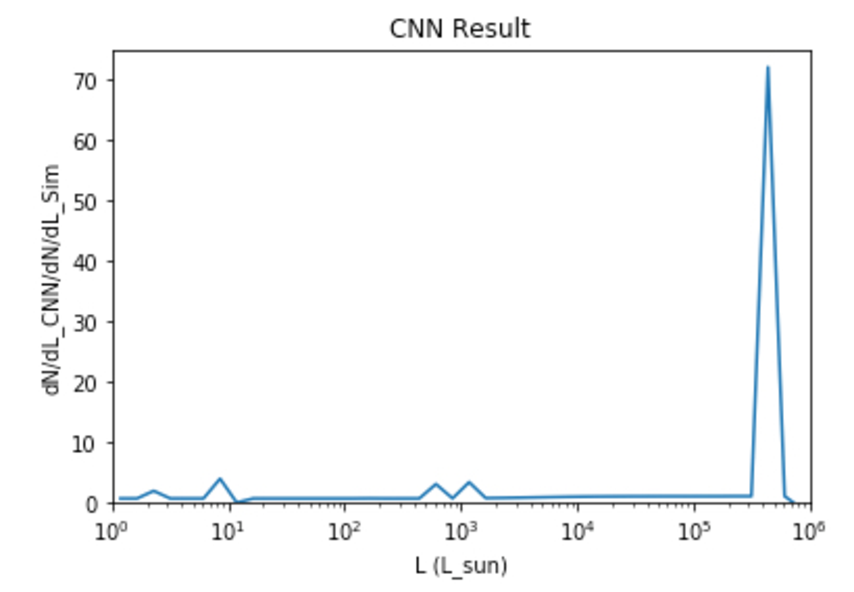
\includegraphics[width=0.8\textwidth]{CNN_4_layer_ratio.pdf}
				\caption{Plot showing the ratio of the CNN luminosity function over the underlying luminosity function.}
				\label{fig:CNN_4_layer_ratio}
			\end{figure}

			\begin{figure}[H]
				\centering
				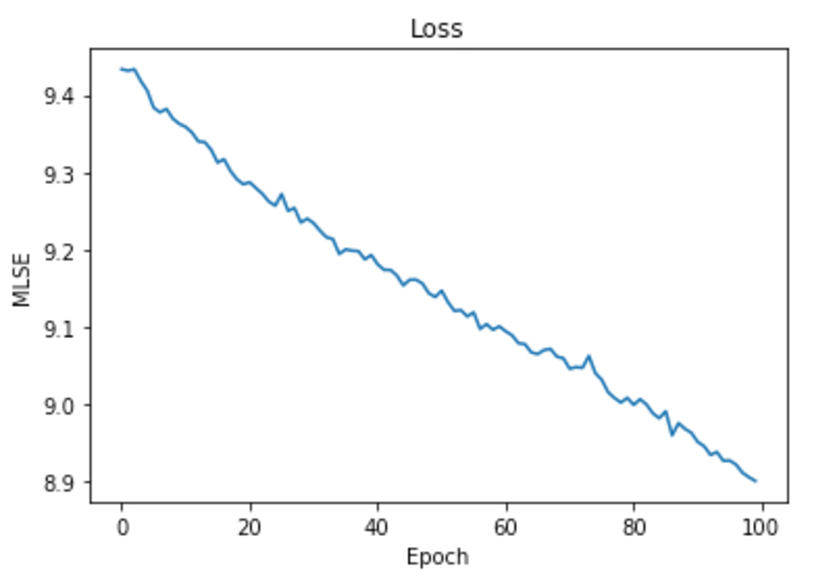
\includegraphics[width=0.8\textwidth]{CNN_4_layer_history_mlse.pdf}
				\caption{Plot showing loss history of the 4 layer CNN that was trained on the full luminosity function.  The loss function that was used was the mean log squared error}
				\label{fig:CNN_4_layer_history_mlse}
			\end{figure}

			\begin{figure}[H]
				\centering
				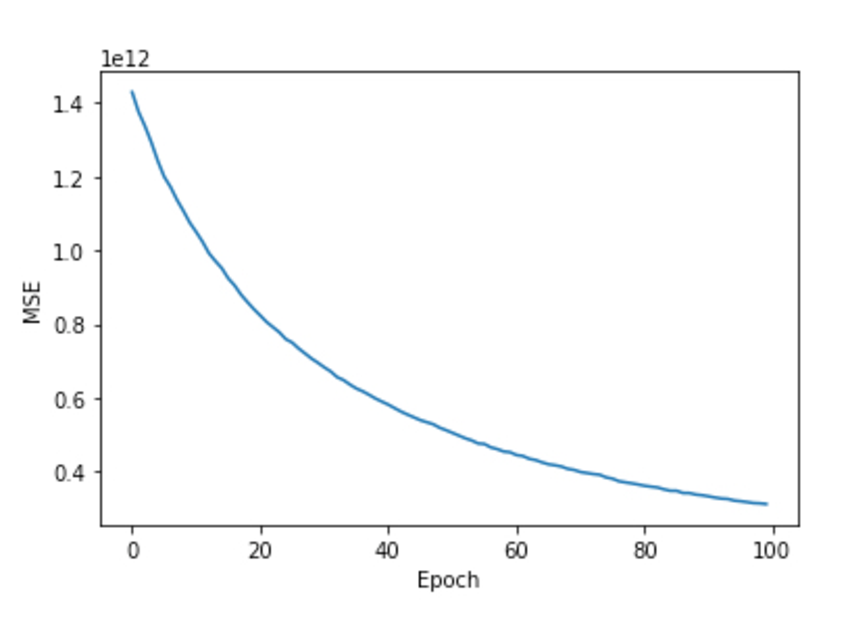
\includegraphics[width=0.8\textwidth]{CNN_4_layer_history_mse.pdf}
				\caption{Plot showing history of the mean squared error metric as a function of epoch.}
				\label{fig:CNN_4_layer_history_mse}
			\end{figure}

		\subsection{5 Layer dN/dL} \label{sec:5directValue}
			I tried making a 5 layer network, but it was much slower and only got around 30 epochs in 48 hours.  It was way too slow to train.  I saved every 20 epochs so not everything was wasted.  \cref{fig:CNN_5_layer} shows how "good" the semi-trained network is and it is pretty bad.  This needs more time.  I'm trying to run it for longer now and see if it will hopefully turn out better then the 4 layer network.

			\begin{figure}[H]
				\centering
				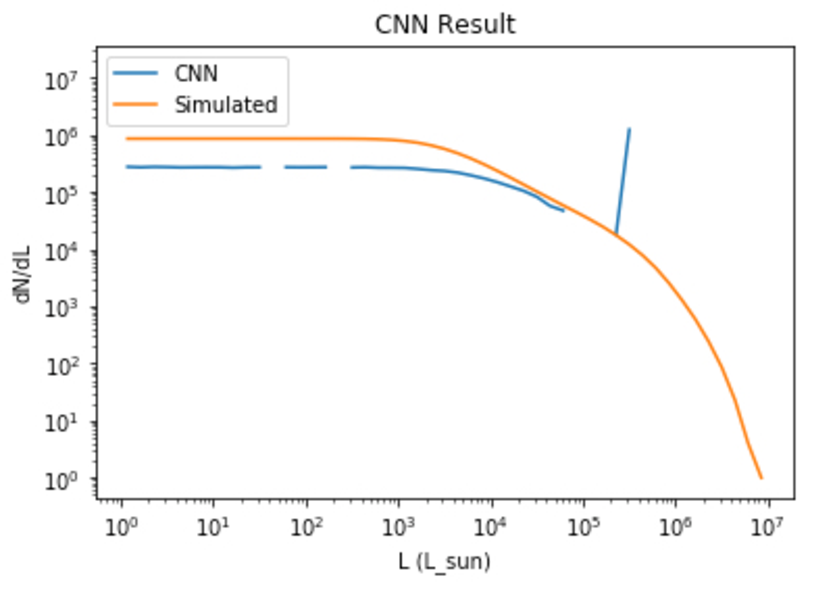
\includegraphics[width=0.8\textwidth]{CNN_5_layer.pdf}
				\caption{Plot showing the comparison of the output of the 5 layer CNN to the expected result of the underlying luminosity function that made the intensity map.}
				\label{fig:CNN_5_layer}
			\end{figure}

	\section{Intensity Mapping CNN (On dN/dL this time)} \label{sec:cnn2}
		The previous shown work was done using the number count instead of the luminosity function.
		\begin{equation}
			N = \int_{L_*}^{\inf} \phi dL
		\end{equation}
		Using the actual luminosity function instead of the number count gives worse results.  I believe this is due to the fact that instead of something that is monotonically decreasing we have to worry about more features.  I think if we converted this to a Fourier space analog and looked at power at different scale we would find more power at lower scales when looking at \(\phi\) rather then \(N\).  In \cref{fig:compare_N_to_phi} we see for a given map the difference between the normalized number counts and normalized luminosity function.  The luminosity function has more features.  These extra features require more training on the part of the CNN.  Training on number counts will be faster and produce better results then the luminosity function.

		\begin{figure}[H]
			\centering
			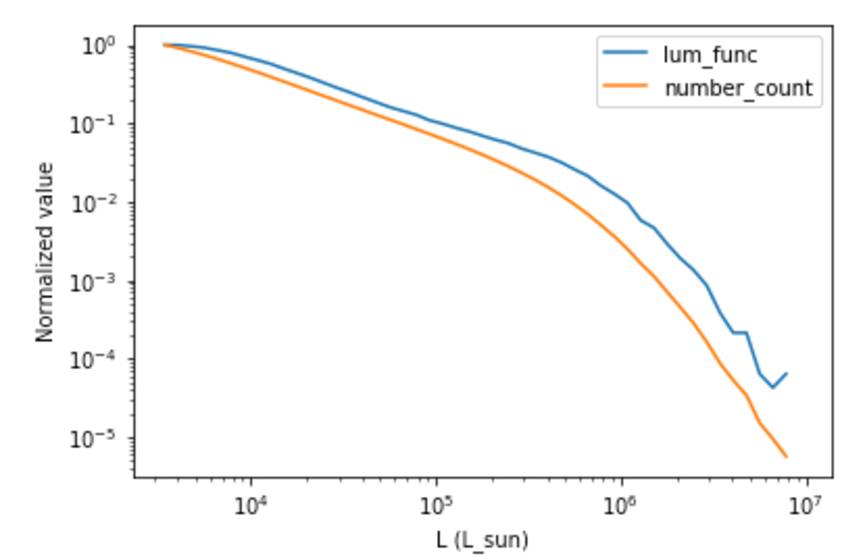
\includegraphics[width=0.8\textwidth]{compare_N_to_phi.pdf}
			\caption{Figure showing the differences between normalized \(N\) and \(\phi\).  The lum func line is \(\phi(L)\) and number count is \(N(L)\).  The main thing to notice is that there are more features in the \(\phi\) curve then the \(N\) curve.}
			\label{fig:compare_N_to_phi}
		\end{figure}

		While training models I get stupid errors that I don't really know every once and a while.  It is some stupid cuda error which makes it very hard to debug and I can't reproduce them.  Just going to throw one of them here so it is in the record.  Line breaks were added by me.

		\begin{verbatim}
			F tensorflow/stream_executor/cuda/cuda_dnn.cc:521] 
			Check failed: cudnnSetTensorNdDescriptor(handle_.get(), 
			elem_type, nd, dims.data(), strides.data()) == 
			CUDNN_STATUS_SUCCESS (3 vs. 0)
			batch_descriptor: {count: 0 feature_map_count: 16 
			spatial: 252 252 96  value_min: 0.000000 
			value_max: 0.000000 layout: BatchDepthYX}
		\end{verbatim} 

		There were also issues with trying to train on \(\phi L\).  I don't know what the network was doing, but it would just start getting nulls, nans or infs for output pretty quickly or it would just give garbage in the end.  It is probably something I'm doing, but maybe the architecture doesn't like the shape of \(\phi L\) as seen in \cref{fig:phi_L}.  it is more complicated then either \(N\) or \(\phi\).

		\begin{figure}[H]
			\centering
			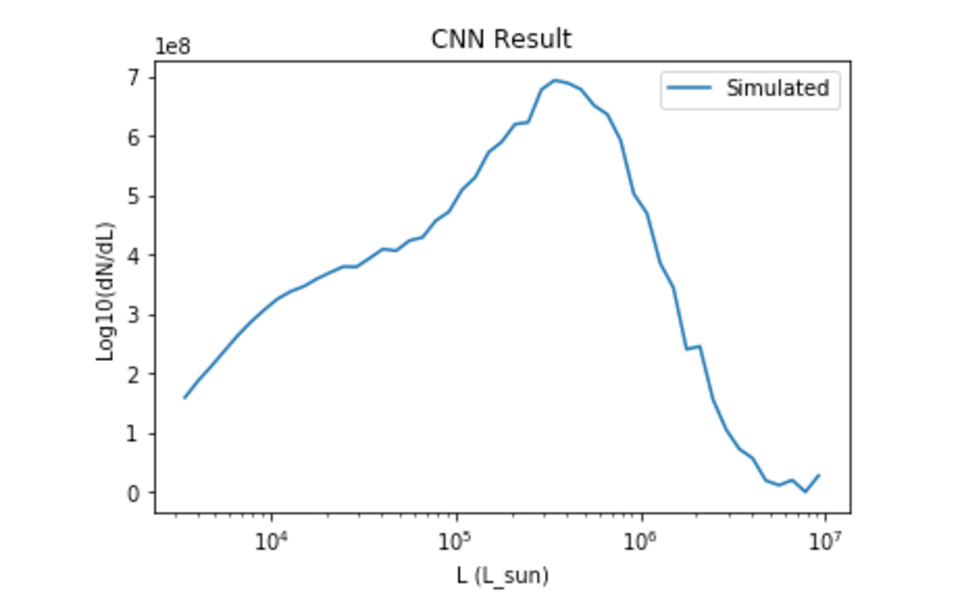
\includegraphics[width=0.8\textwidth]{phi_L.pdf}
			\caption{A generic look at what \(\phi L\) v.s. \(L\) should look like.}
			\label{fig:phi_L}
		\end{figure}

		\subsection{2D v.s. 3D}
			When designing the CNN we have a choice between doing 2D or 3D convolutions.  3D makes things much slower and requires more space.  A comparison between 2D and 3D models can be seen in \cref{fig:2d_vs_3d}.  From the figure it is clear that the 2D model beats the 3D one and the longer running 2D model does best.  The 3D model just doesn't look good.  I can't get it to actually work for the log values.  I don't have a model for 5 layers due to it failing at some point while running.

			\begin{figure}[H]
				\centering
				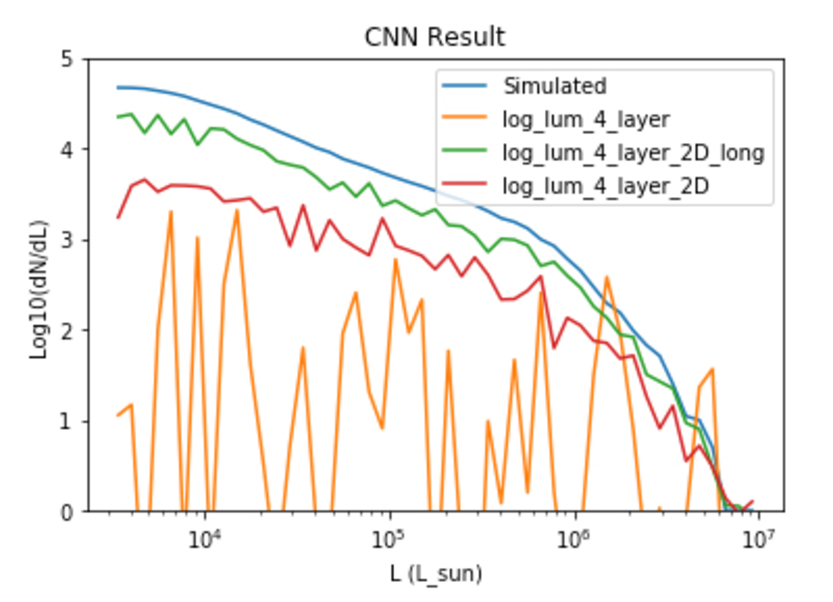
\includegraphics[width=0.8\textwidth]{2d_vs_3d.pdf}
				\caption{A comparison between three different models.  For two of them the difference between them was that one was with 3D convolutions and the other with 2D ones.  Their epochs were roughly the same number of evaluations and they had the same number of epochs.  The long model was run with more evaluations per epoch rather then more epochs.}
				\label{fig:2d_vs_3d}
			\end{figure}

			It seems, at least for the log values, that it is better to go with the 2D convolutions.  It is faster, more space efficient and gives better results.

			We can compare the loss history of the 2D and 3D models in \cref{fig:log_lum_4_layer_2D_history,fig:log_lum_4_layer_history} to try and see what's going on.  The history for the 3D one is garbage.  The validation loss never goes down.  I don't fully understand what is happening.  Naively this would mean that it is memorizing the training data and not knowing the validation data.  The issue with this is that if I run the model on data that should have been training data it still returns garbage.  The 2D model is better.  The validation data does improve, but it stalls out around halfway through and doesn't improve much anymore.  It does show learning though.

			\begin{figure}[H]
				\centering
				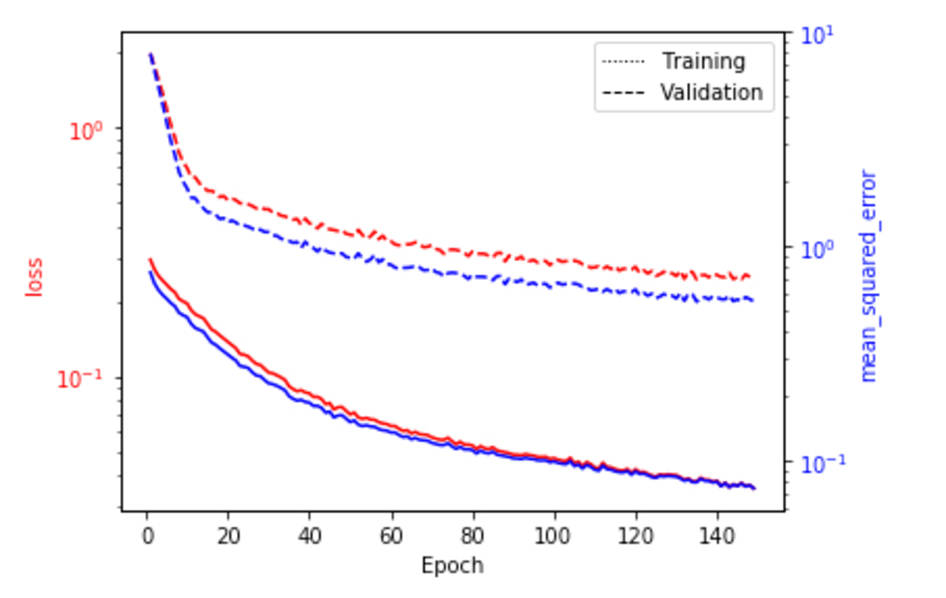
\includegraphics[width=0.8\textwidth]{log_lum_4_layer_2D_history.pdf}
				\caption{Loss history of the training of the 4 layer, 2D and log valued model.  Note that training data is actually the solid line not what the legend says.}
				\label{fig:log_lum_4_layer_2D_history}
			\end{figure}

			\begin{figure}[H]
				\centering
				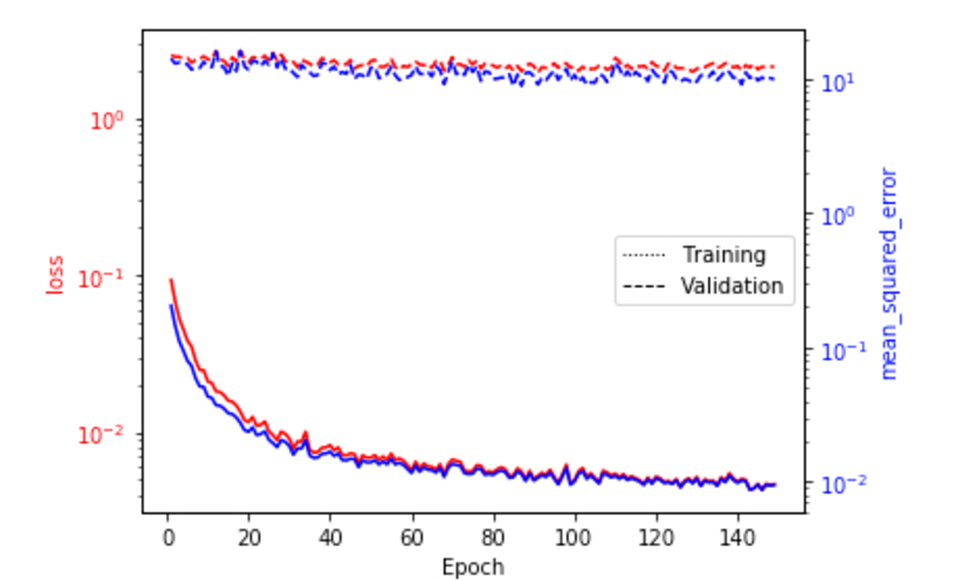
\includegraphics[width=0.8\textwidth]{log_lum_4_layer_history.pdf}
				\caption{Loss history of the training of the 4 layer and log valued model.  Note that training data is actually the solid line not what the legend says.}
				\label{fig:log_lum_4_layer_history}
			\end{figure}

			I don't have models in both 2D and 3D for testing against \(\phi\) or \(\phi L\) to see how they differ between the dimensions.

		\subsection{What is actually working?} \label{sec:wiaw}

			\begin{figure}[H]
				\centering
				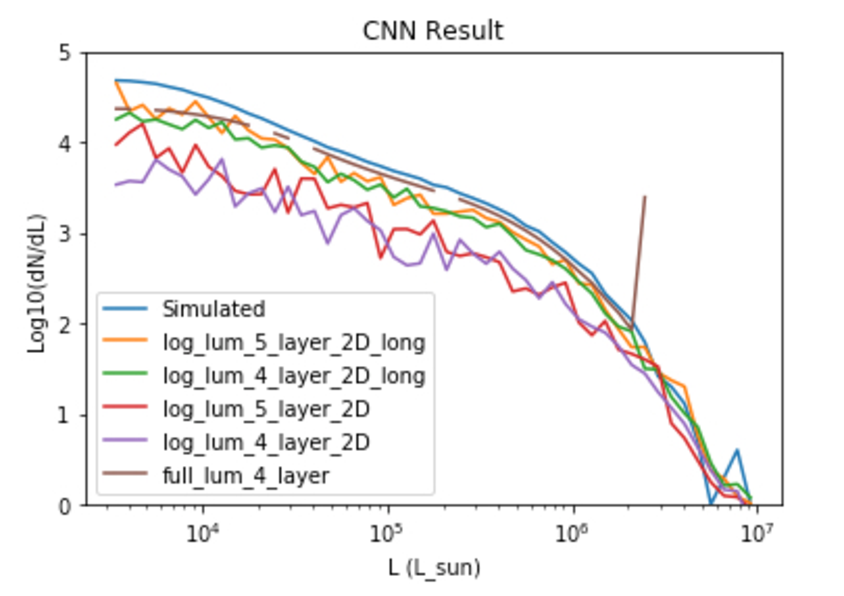
\includegraphics[width=0.8\textwidth]{compare_models.pdf}
				\caption{Comparison of the output from a few different models.}
				\label{fig:compare_models}
			\end{figure}

			Now lets try to figure out what is working and what we should be continuing on with.  \cref{fig:compare_models} shows the output from a few different models for a single map.  Note that not every model was trained on log data, but it is presented in log space now.  A few things become apparent by looking at the curves.  First is that the longer training models did better then the less trained models.  This is seen comparing the 4 and 5 layer 2D log data v.s. the long version of those.  \dnp{Who could have guessed this?}  The next thing to notice is that the 4 layer network trained on the full luminosity function isn't bad.  I would have expected this to be awful.  The range of values it needs to get is very large, but it was one of the best trained models.  It does have some holes in it's range which we saw earlier for a similar model in \cref{fig:CNN_4_layer}.  I don't know why those things are appearing, but they do.  \dnp{Maybe more training will help?}  

			More models were tested then what is in the figure, but the best were shown.

			In \cref{fig:compare_models_ratio} we can look at the ratio of model output to expected output as a function of \(L\).  In this figure we see that the 4 layer full luminosity function model is best at times with the 5 layer 2D log value one behind that and the 4 layer version of the previous model slightly worse off.

			\begin{figure}[H]
				\centering
				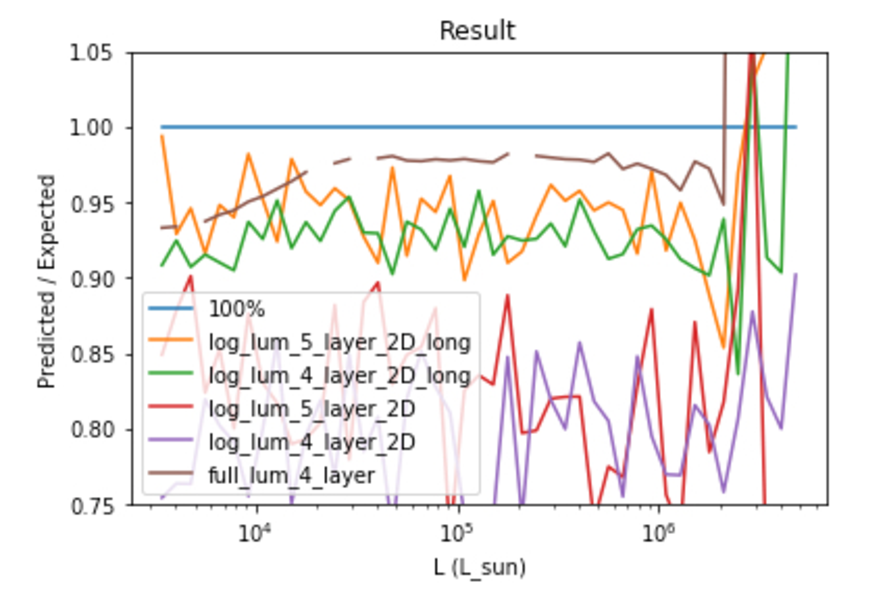
\includegraphics[width=0.8\textwidth]{compare_models_ratio.pdf}
				\caption{Comparison of the ratio of output to expected value from a few different models.}
				\label{fig:compare_models_ratio}
			\end{figure}

			Again it is useful to look at the training history.  When comparing the 4 layer and 5 layer histories in \cref{fig:log_lum_4_layer_2D_model_long_history,fig:log_lum_5_layer_2D_model_long_history} we see that there is a big gap between the training in validation for 4 layers, but not for 5 layers.  It might be that the network isn't big enough with 4 layers to learn as fast as it can.  The 5 layer network learns very nicely and doesn't appear to be leveling out yet when the training ended.  I don't know how, but somehow training in 3D gave a terrible history which can be seen in \cref{fig:full_lum_4_layer_model_history}.  The training and validation loss data are mostly the same after about 40 epochs, but it oscillates which is weird.  The mse error improves for some reason even though it isn't being trained on that and the loss isn't really improving.

			\begin{figure}[H]
				\centering
				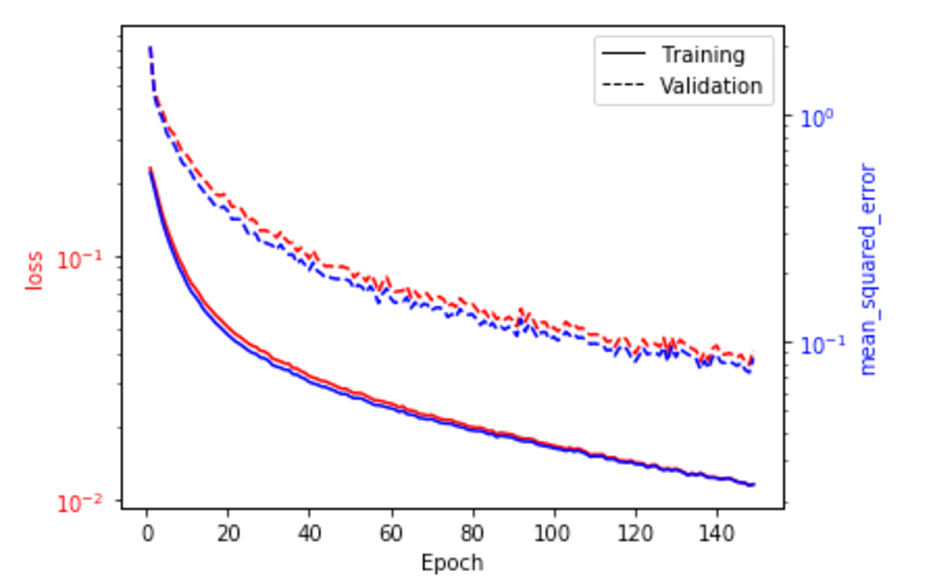
\includegraphics[width=0.8\textwidth]{log_lum_4_layer_2D_model_long_history.pdf}
				\caption{Loss history of the training of the 4 layer 2D log valued model.}
				\label{fig:log_lum_4_layer_2D_model_long_history}
			\end{figure}

			\begin{figure}[H]
				\centering
				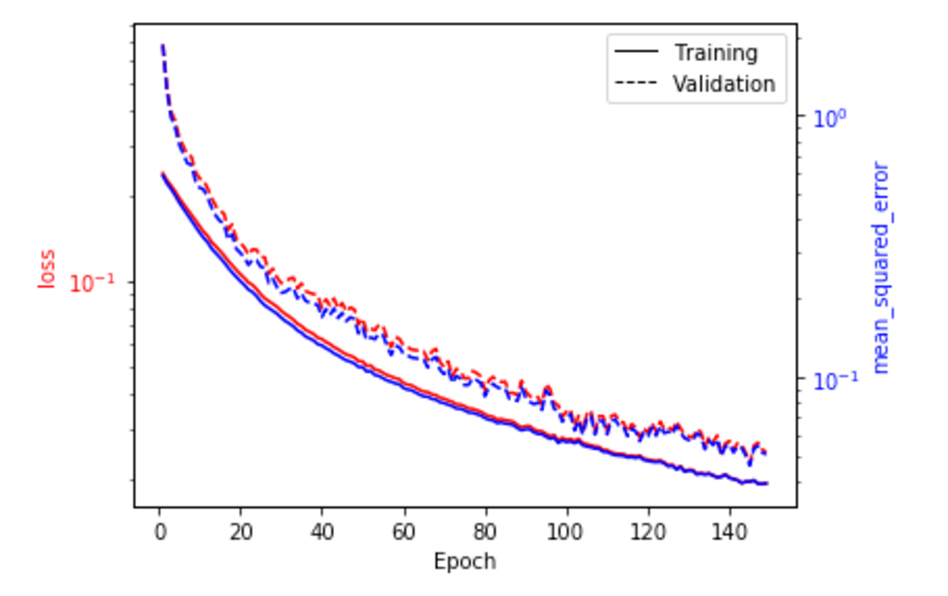
\includegraphics[width=0.8\textwidth]{log_lum_5_layer_2D_model_long_history.pdf}
				\caption{Loss history of the training of the 5 layer 2D log valued model.}
				\label{fig:log_lum_5_layer_2D_model_long_history}
			\end{figure}

			\begin{figure}[H]
				\centering
				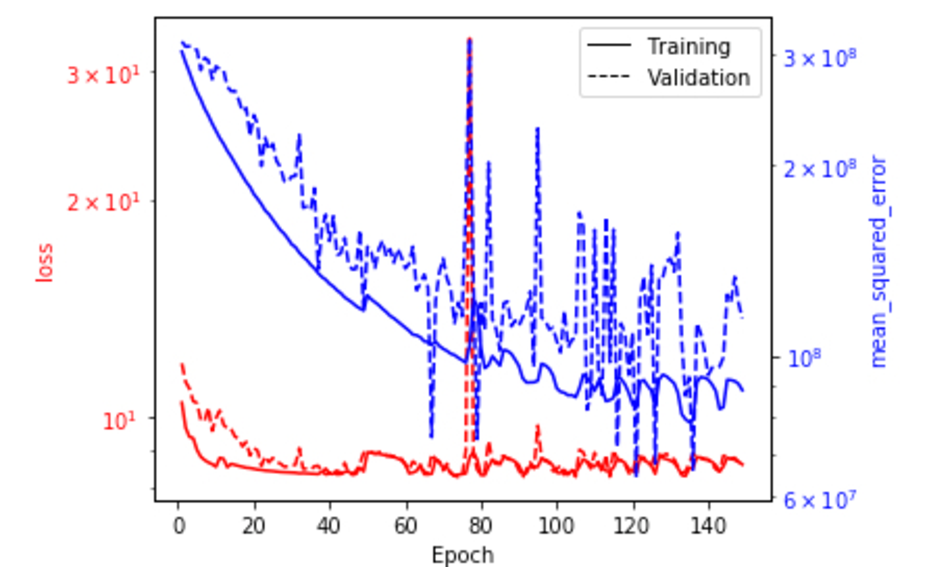
\includegraphics[width=0.8\textwidth]{full_lum_4_layer_model_history.pdf}
				\caption{Loss history of the training of the 4 layer full valued model.}
				\label{fig:full_lum_4_layer_model_history}
			\end{figure}

	\section{Finalizing the architectures} \label{sec:arch}
		\subsection{No Noise} \label{sec:third_batch}
			The architecture of the model needs to be finalized.  The last things to look at are really
			\begin{enumerate}
				\item log v.s. normal map input values

				\item \(\phi\) v.s. \(N\)

				\item How many layers and filters can the gpu handle

				\item Any changes to hyper parameters?
			\end{enumerate}

			Note that I know realized that whenever I have been using \(\phi\) in the second batch of testing I have only been using \(dN\).  I've only been considering the differential amount of sources in a bin.  Because I am using log bins this should be the same as \(dN/d\log L\) up to a constant amplitude difference.

			\cref{fig:arch_compare_n,fig:arch_compare_n_ratio,fig:arch_compare_dn,fig:arch_compare_dn_ratio} show the difference between models that vary, number of layers, number of base filters, log input v.s. normal inputs, dN v.s. N and kernel size for convolutions.  The base number of filters was 32 and was used by everything but the most\_filters model.  The most\_filters model used 128 filters, but ran out of memory when training for the second time so only trained half as long as the other models.  Because there is a convolution layer (that acts as a pooling layer) between normal convolution layers there is a max number of layers.  After 5 layers the remaining image is only 4x4 so convolutions using our original 5x5 filter just gets all information at once.  The way around this is to use a kernel size of 3x3 instead.  The 6 layer model uses 3x3 kernels.  There was also a test of a 5 layer model with a 3x3 kernel.

			The output for the model trained on N gives weird results when displaying \(\log_{10} dN\) because it gets negative values that don't log well.  What we see in these figures is that more filters and more layers are better then less although they end up at pretty much the same accuracy.  We also see that the model trained on N is good at predicting N.  Models are generally better at predicting N and with less noise then dN.

			\begin{figure}[H]
				\centering
				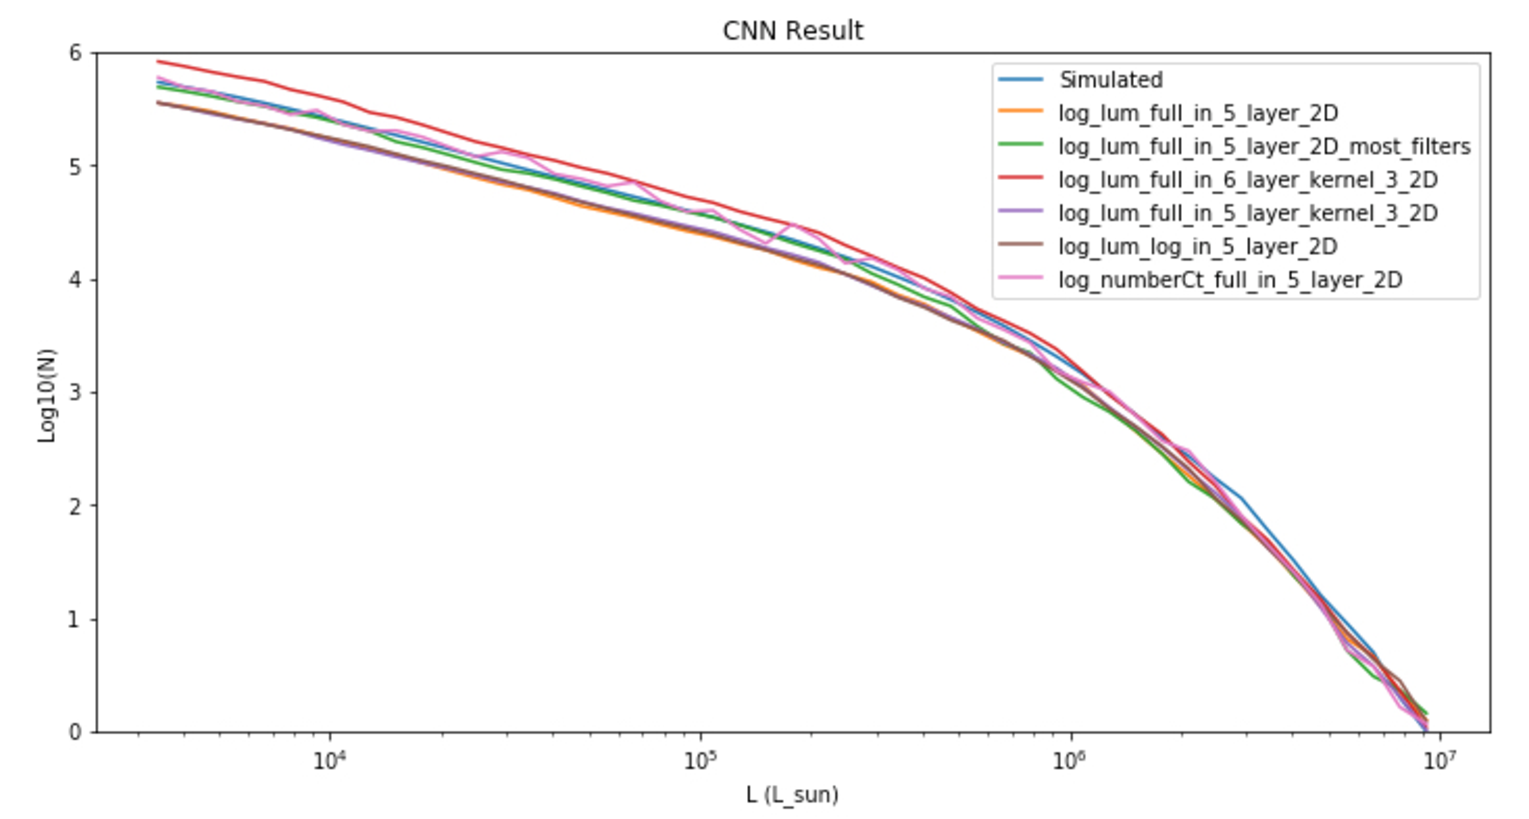
\includegraphics[width=1.0\textwidth]{arch_compare_n.pdf}
				\caption{Output of different CNN architectures for N.}
				\label{fig:arch_compare_n}
			\end{figure}

			\begin{figure}[H]
				\centering
				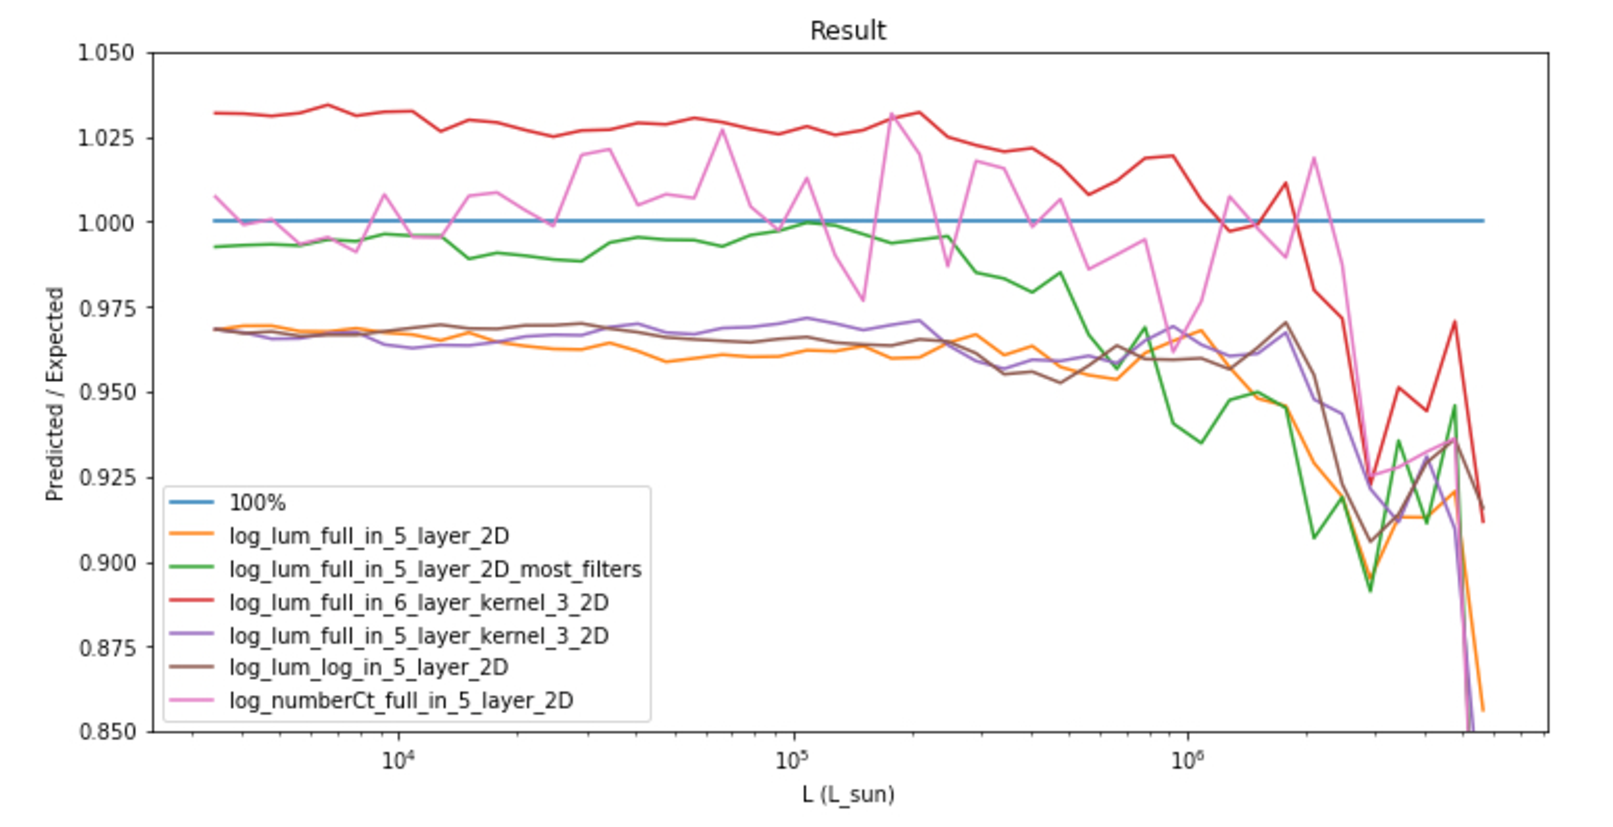
\includegraphics[width=1.0\textwidth]{arch_compare_n_ratio.pdf}
				\caption{Same as \cref{fig:arch_compare_n}, but showing ratio of CNN output to underlying value instead of raw values.}
				\label{fig:arch_compare_n_ratio}
			\end{figure}

			\begin{figure}[H]
				\centering
				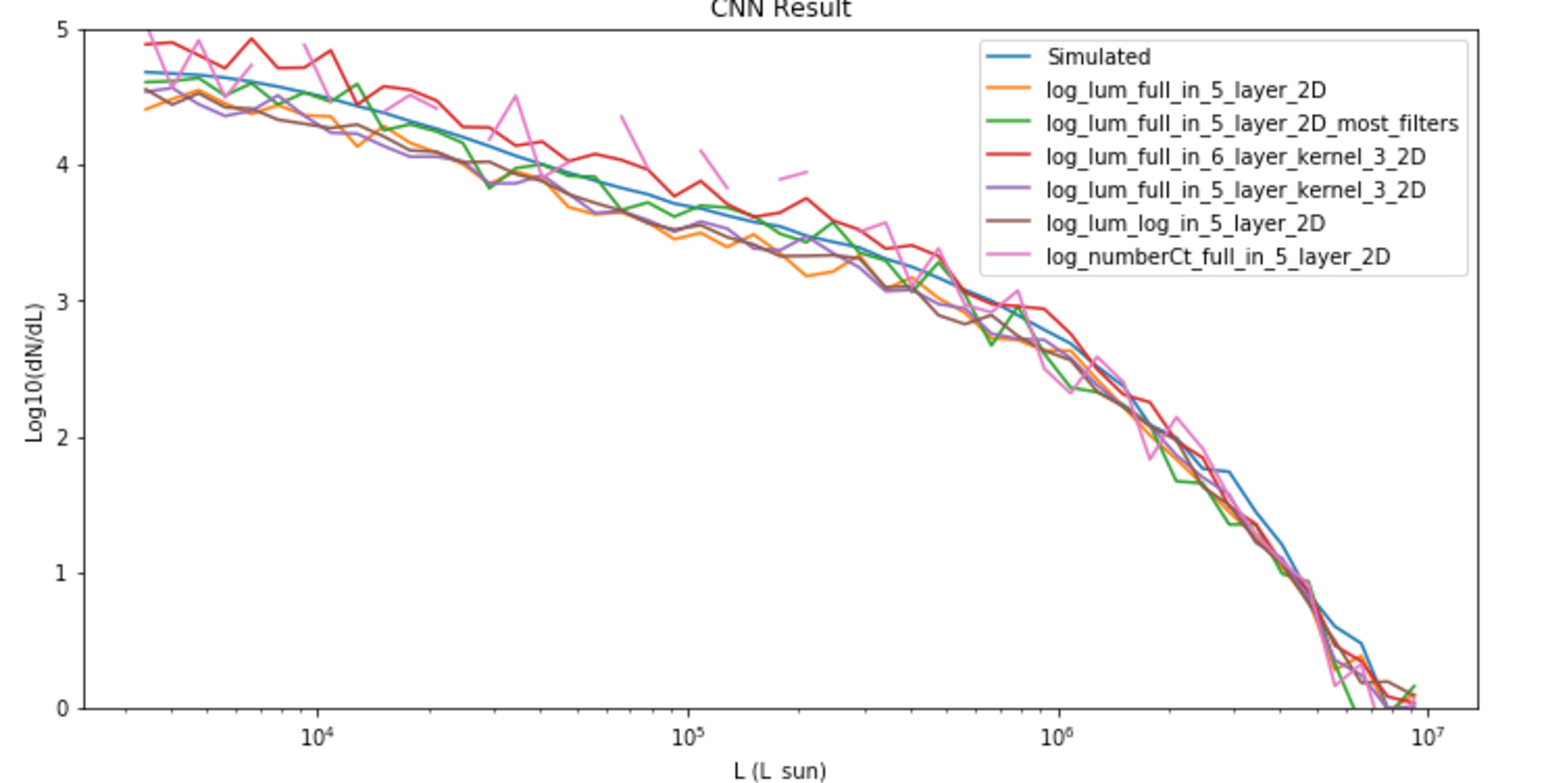
\includegraphics[width=1.0\textwidth]{arch_compare_dn.pdf}
				\caption{Output of different CNN architectures for dN.}
				\label{fig:arch_compare_dn}
			\end{figure}

			\begin{figure}[H]
				\centering
				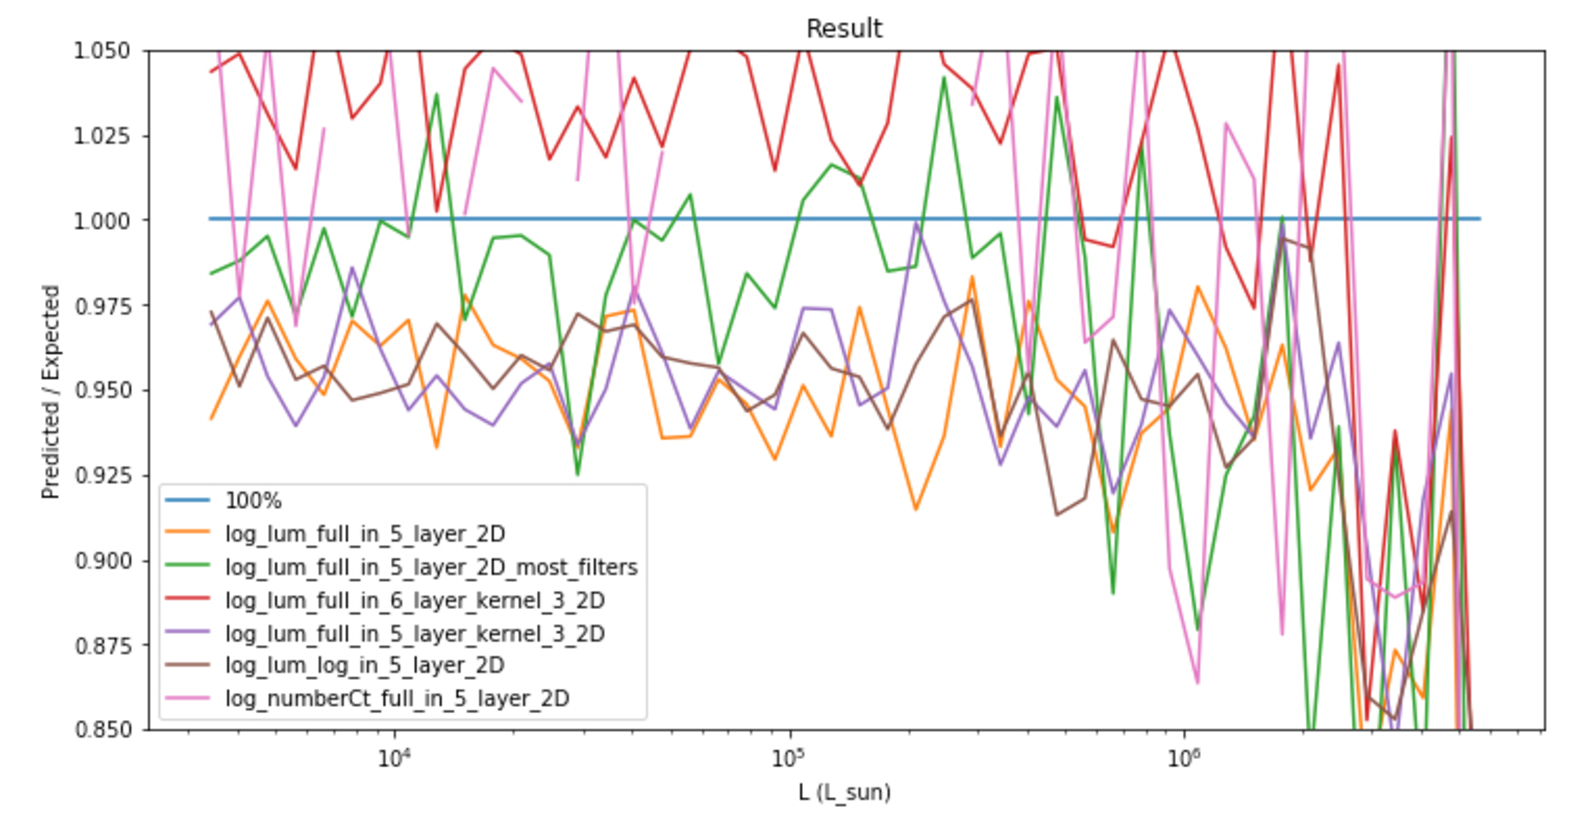
\includegraphics[width=1.0\textwidth]{arch_compare_dn_ratio.pdf}
				\caption{Same as \cref{fig:arch_compare_dn}, but showing ratio of CNN output to underlying value instead of raw values.}
				\label{fig:arch_compare_dn_ratio}
			\end{figure}

			The loss from training and validation from a few models are shown in \cref{fig:log_lum_full_in_5_layer_2D_history,fig:log_numberCt_full_in_5_layer_2D_history,fig:log_lum_full_in_5_layer_2D_most_filters_history,fig:log_lum_full_in_6_layer_kernel_3_2D_history}.  The validation loss being less than the training loss is interesting.  This could be due to dropout while training.  While training 20\% of the neurons don't fire as a way to help prevent over-fitting.  It also means that the CNN isn't at it's best while training.  Validation data is taken without dropout so it can be better.  The weird discontinuities at the 100th epoch are due to the model being trained again.  I only had enough time to train for 100 epochs before time out so I had to resume and in doing so it did something.  One should be careful about comparing the log luminosity models to the number count models because they are looking at different things so different values are to be expected.

			\begin{figure}[H]
				\centering
				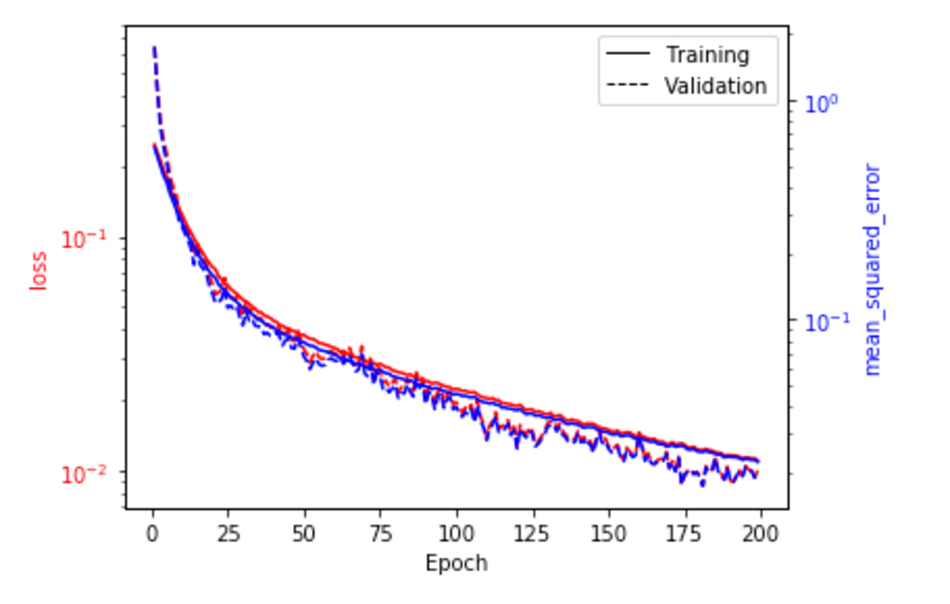
\includegraphics[width=0.8\textwidth]{log_lum_full_in_5_layer_2D_history.pdf}
				\caption{Loss history of the training of the log\_lum\_full\_in\_5\_layer\_2D model.}
				\label{fig:log_lum_full_in_5_layer_2D_history}
			\end{figure}

			\begin{figure}[H]
				\centering
				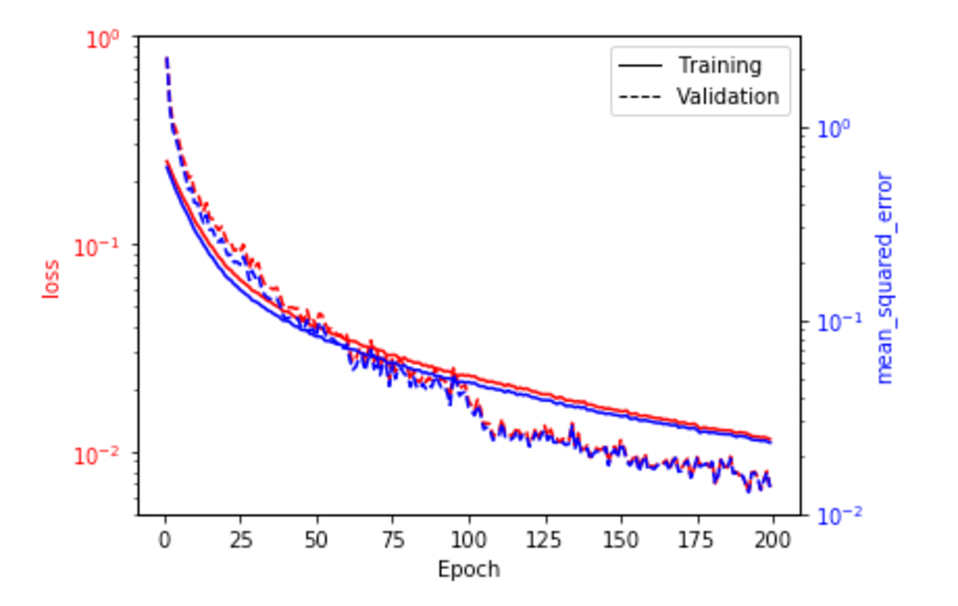
\includegraphics[width=0.8\textwidth]{log_numberCt_full_in_5_layer_2D_history.pdf}
				\caption{Loss history of the training of the log\_numberCt\_full\_in\_5\_layer\_2D model.}
				\label{fig:log_numberCt_full_in_5_layer_2D_history}
			\end{figure}

			\begin{figure}[H]
				\centering
				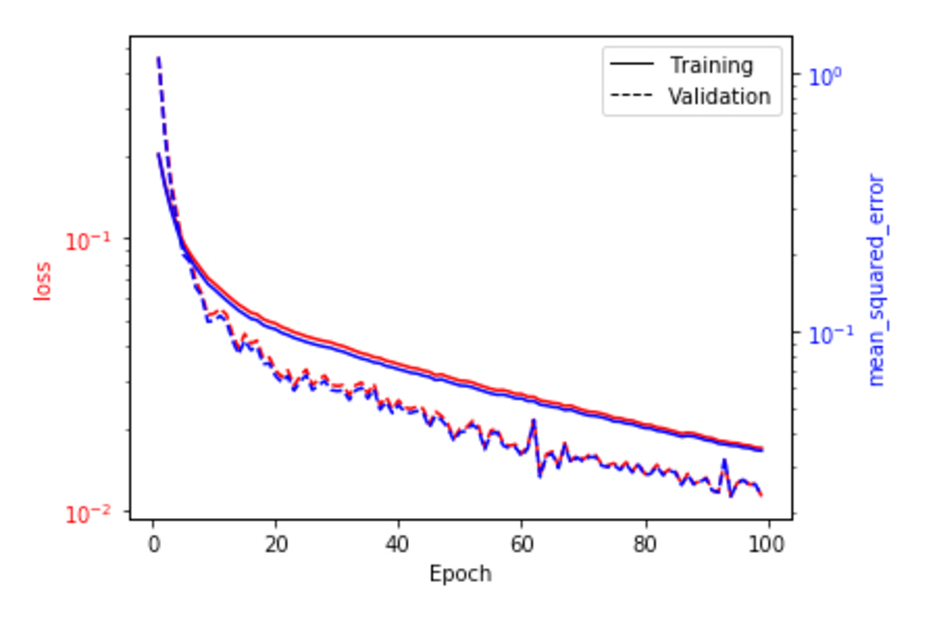
\includegraphics[width=0.8\textwidth]{log_lum_full_in_5_layer_2D_most_filters_history.pdf}
				\caption{Loss history of the training of the log\_lum\_full\_in\_5\_layer\_2D\_most\_filters model.}
				\label{fig:log_lum_full_in_5_layer_2D_most_filters_history}
			\end{figure}

			\begin{figure}[H]
				\centering
				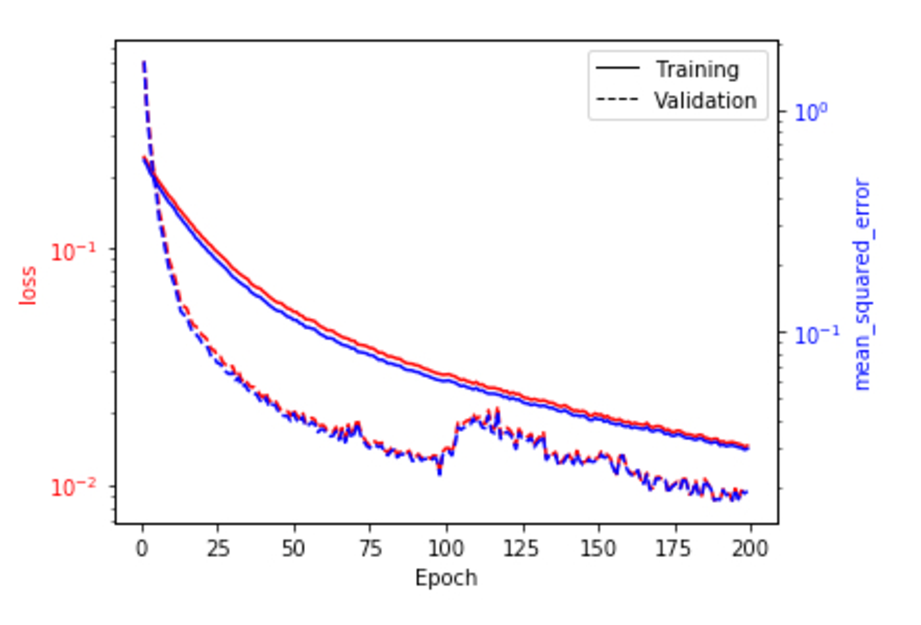
\includegraphics[width=0.8\textwidth]{log_lum_full_in_6_layer_kernel_3_2D_history.pdf}
				\caption{Loss history of the training of the log\_lum\_full\_in\_6\_layer\_kernel\_3\_2D model.}
				\label{fig:log_lum_full_in_6_layer_kernel_3_2D_history}
			\end{figure}

		\subsection{Adding Noise} \label{sec:noise}

			Testing models on perfect information is all good and dandy, but we want to test our models against more realistic scenarios.  In https://arxiv.org/abs/1808.07487 they try to get the luminosity function (\(\phi L\)) from intensity maps using an MCMC and power spectra.  They also include an 11 \(\mu K\) white noise to their maps so it would be good to compare to their work.  \cref{fig:arch_compare_noise_n,fig:arch_compare_noise_n_ratio,fig:arch_compare_noise_dn,fig:arch_compare_noise_dn_ratio} are similar to \cref{fig:arch_compare_n,fig:arch_compare_n_ratio,fig:arch_compare_dn,fig:arch_compare_dn_ratio} except the map (it is the same exact map) was loaded with 11 \(\mu K\) of white noise.

			What we see is that most models get worse as in they predict less N or dN for all luminosities, but the 6 layer one gets much better because it originally over predicted values.  Increasing the noise by a factor of 10 to 100 \(\mu K\) does not change model predictions that much.  There is some variation because the noise varies whenever the map is loaded, but adding noise makes the 6 layer model better.  All of the other models bunch together.  This was not training on noise or anything, this is just taking the models we trained on perfect data and just putting noise into the maps when we want a prediction.  

			\begin{figure}[H]
				\centering
				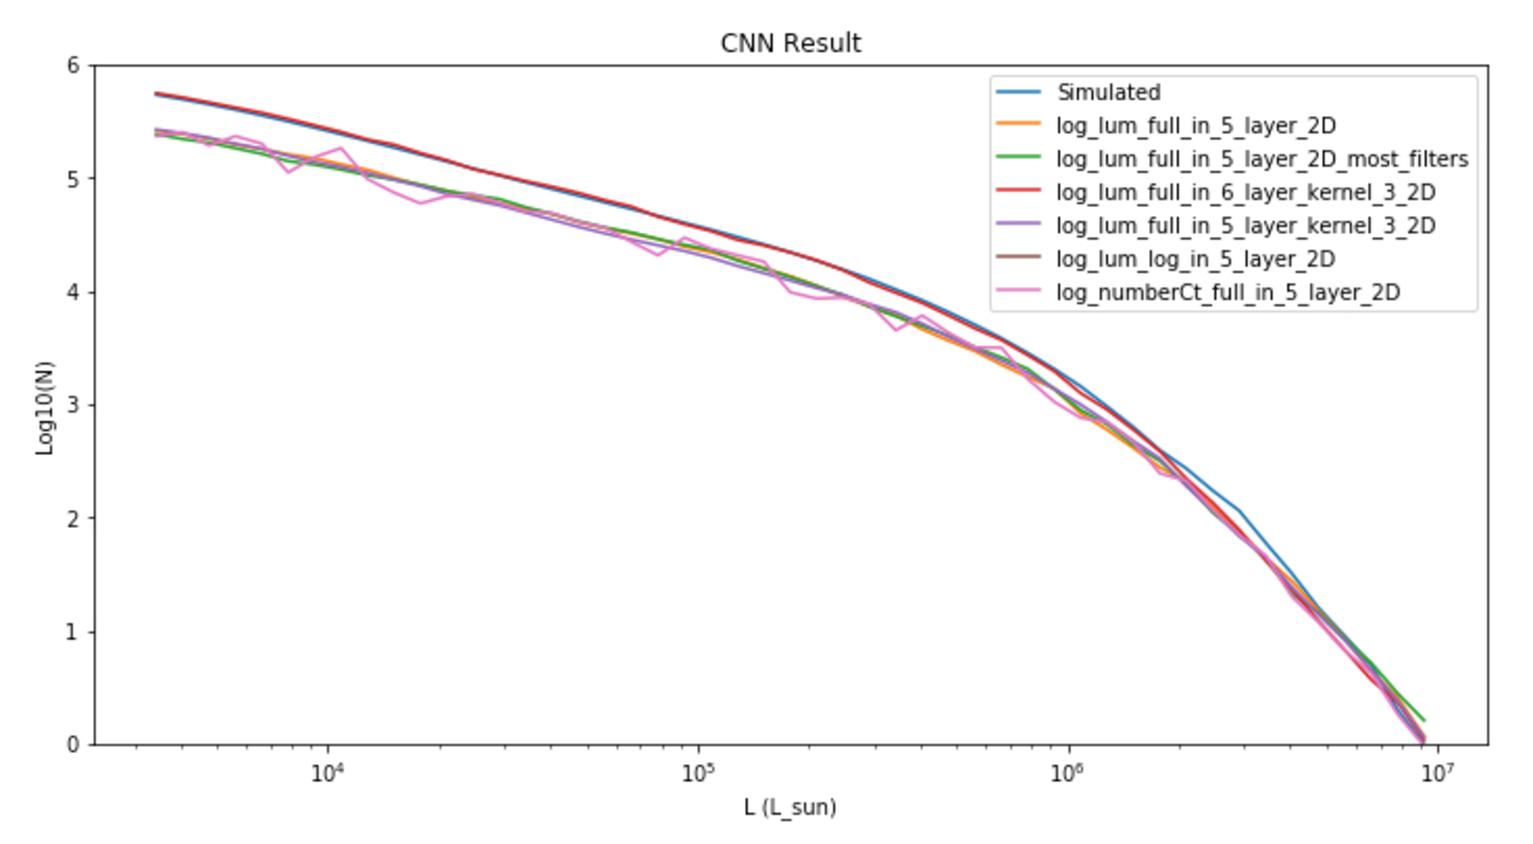
\includegraphics[width=1.0\textwidth]{arch_compare_noise_n.pdf}
				\caption{Output of different CNN architectures for N with 10 \(\mu K\) white noise.}
				\label{fig:arch_compare_noise_n}
			\end{figure}

			\begin{figure}[H]
				\centering
				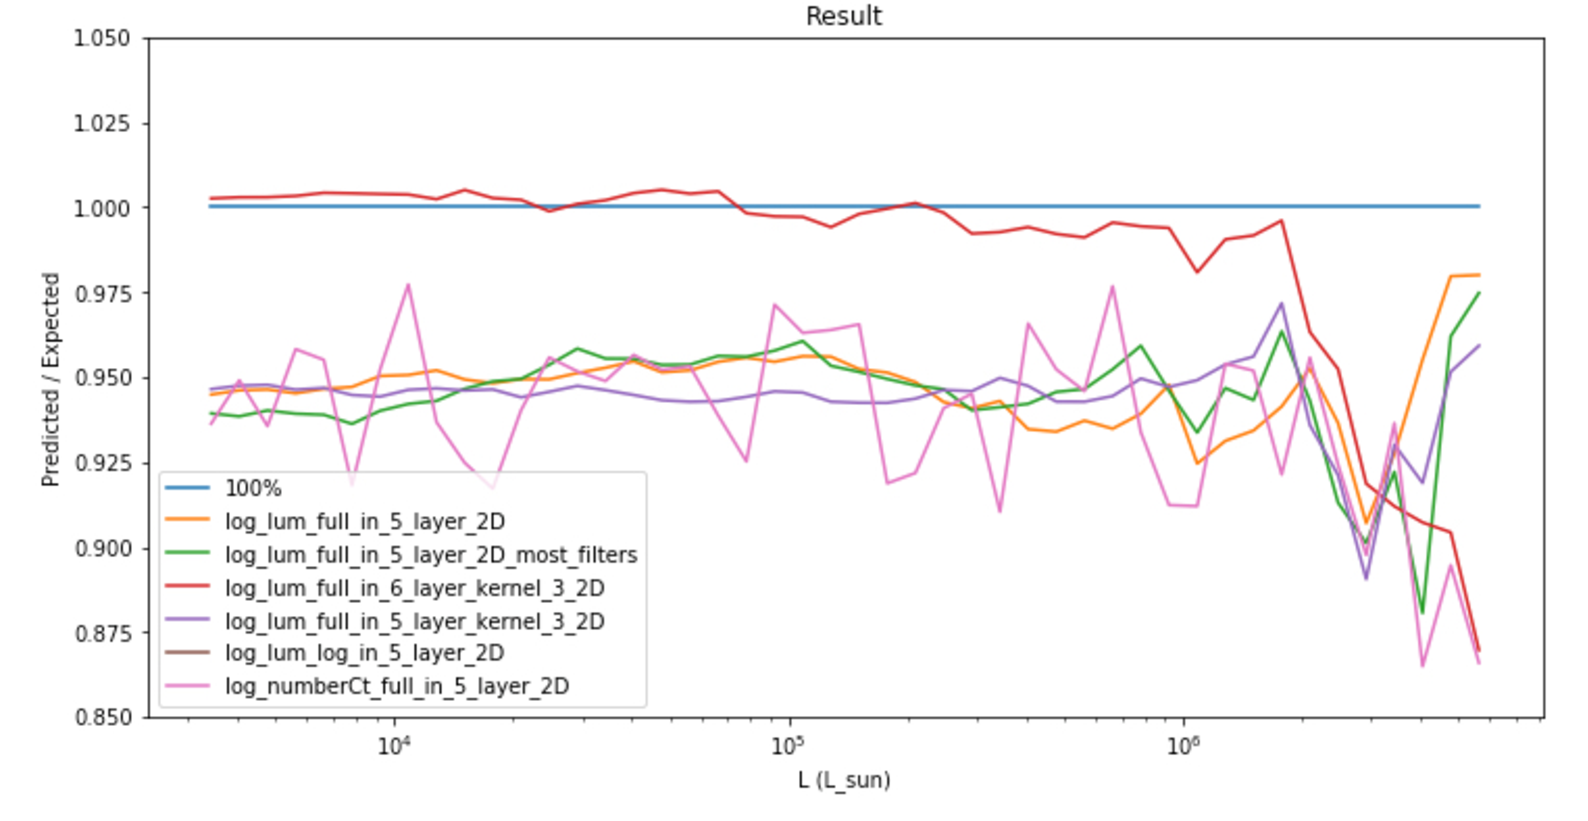
\includegraphics[width=1.0\textwidth]{arch_compare_noise_n_ratio.pdf}
				\caption{Same as \cref{fig:arch_compare_noise_n}, but showing ratio of CNN output to underlying value instead of raw values.}
				\label{fig:arch_compare_noise_n_ratio}
			\end{figure}

			\begin{figure}[H]
				\centering
				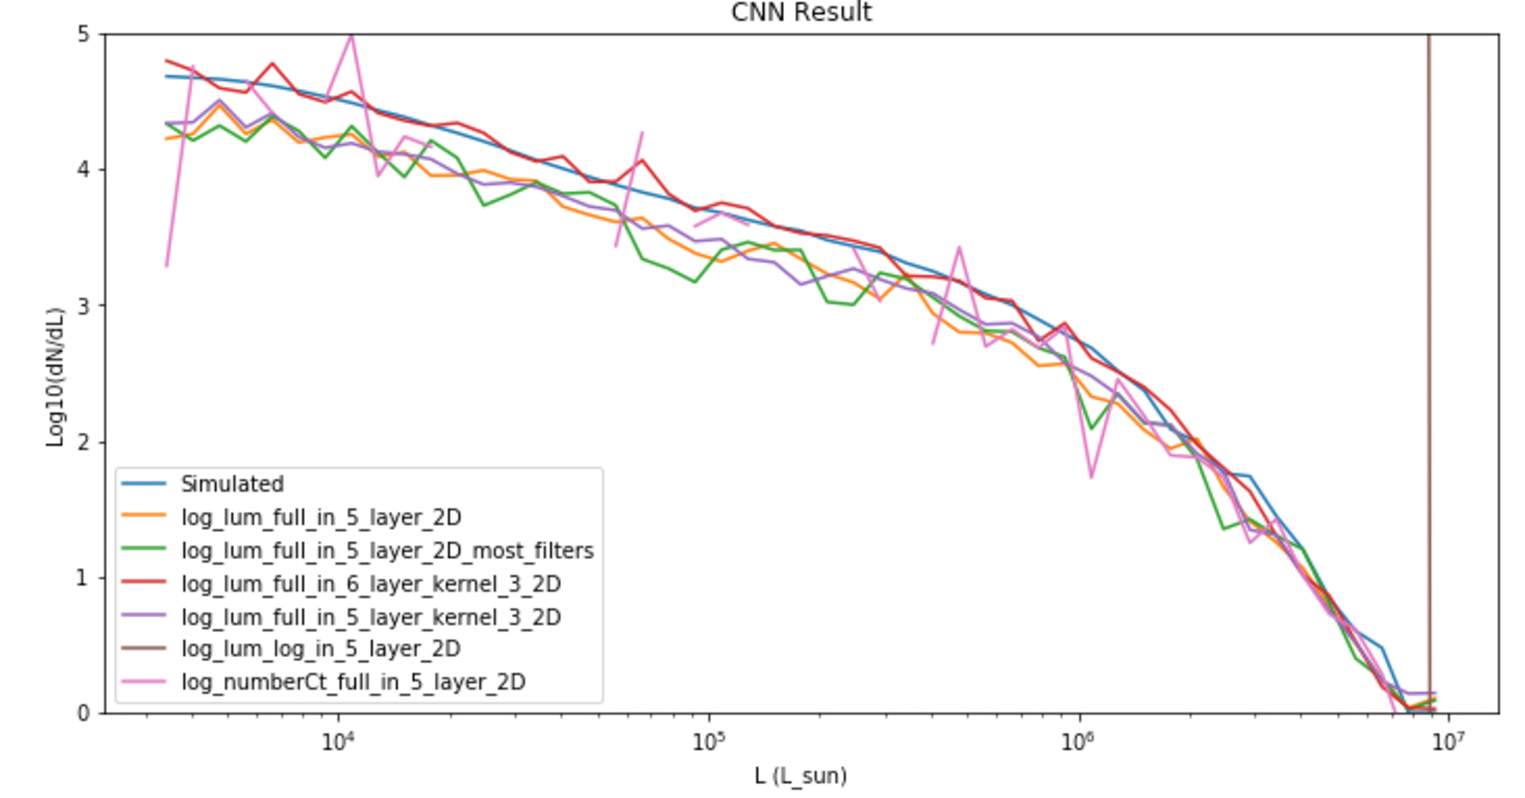
\includegraphics[width=1.0\textwidth]{arch_compare_noise_dn.pdf}
				\caption{Output of different CNN architectures for dN with 11 \(\mu K\) white noise.}
				\label{fig:arch_compare_noise_dn}
			\end{figure}

			\begin{figure}[H]
				\centering
				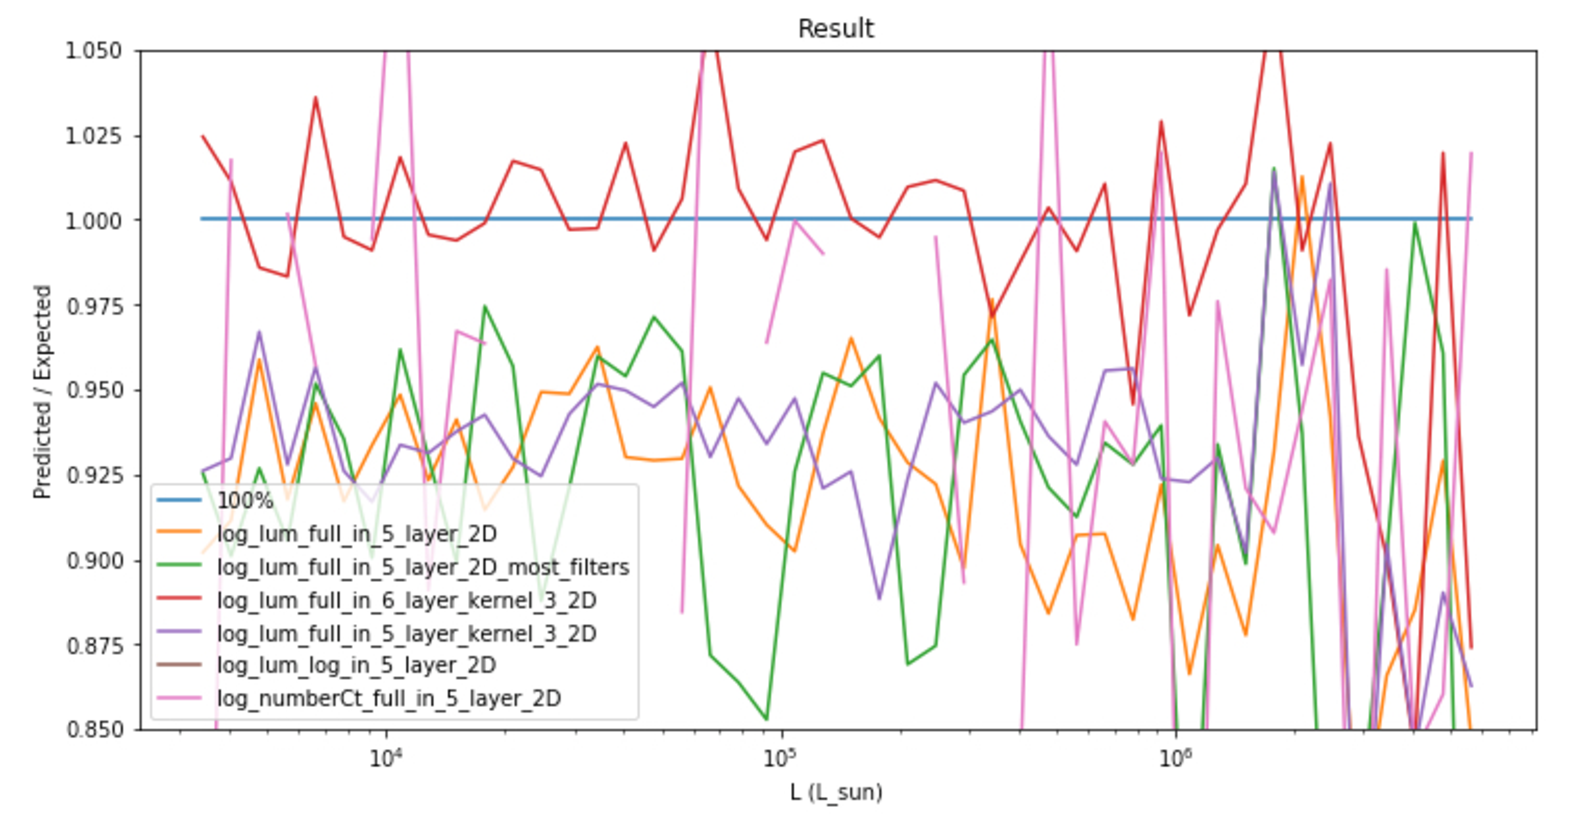
\includegraphics[width=1.0\textwidth]{arch_compare_noise_dn_ratio.pdf}
				\caption{Same as \cref{fig:arch_compare_noise_dn}, but showing ratio of CNN output to underlying value instead of raw values.}
				\label{fig:arch_compare_noise_dn_ratio}
			\end{figure}

	\section{Compare to \href{https://arxiv.org/pdf/1808.07487.pdf}{COMAP power spectrum luminosity method} work} \label{sec:power_compare}
		The work in \cref{sec:arch} points to wanting to have more layers and more filters.  There was no reason to go beyond 6 layers because of the fact that we would not be able to convolve anything in the 7th layer.  More than 64 starting filters would lead to memory issues so we decided to only test 32 and 64 initial filters.  Hyperparameters were still not messed with.  \cref{fig:power_compare_dn,fig:power_compare_dn_ratio,fig:power_compare_noise_dn,fig:power_compare_noise_dn_ratio} show the results of 200 epochs of training 6 layer models with a kernel size of 3 with starting size of 32 or 64 filters as well as training with noise or not.  The plots show the usual things of comparing the output for N and dN v.s. the underlying values and then looking at the ratio of predicted to underlying.  What we see is that the 64 filters doesn't do the best.  Noise actually improves the 32 filter model, but doesn't do much for the 64 filter models.  It seems like 32 filters is a good amount to have.

		\begin{figure}[H]
				\centering
			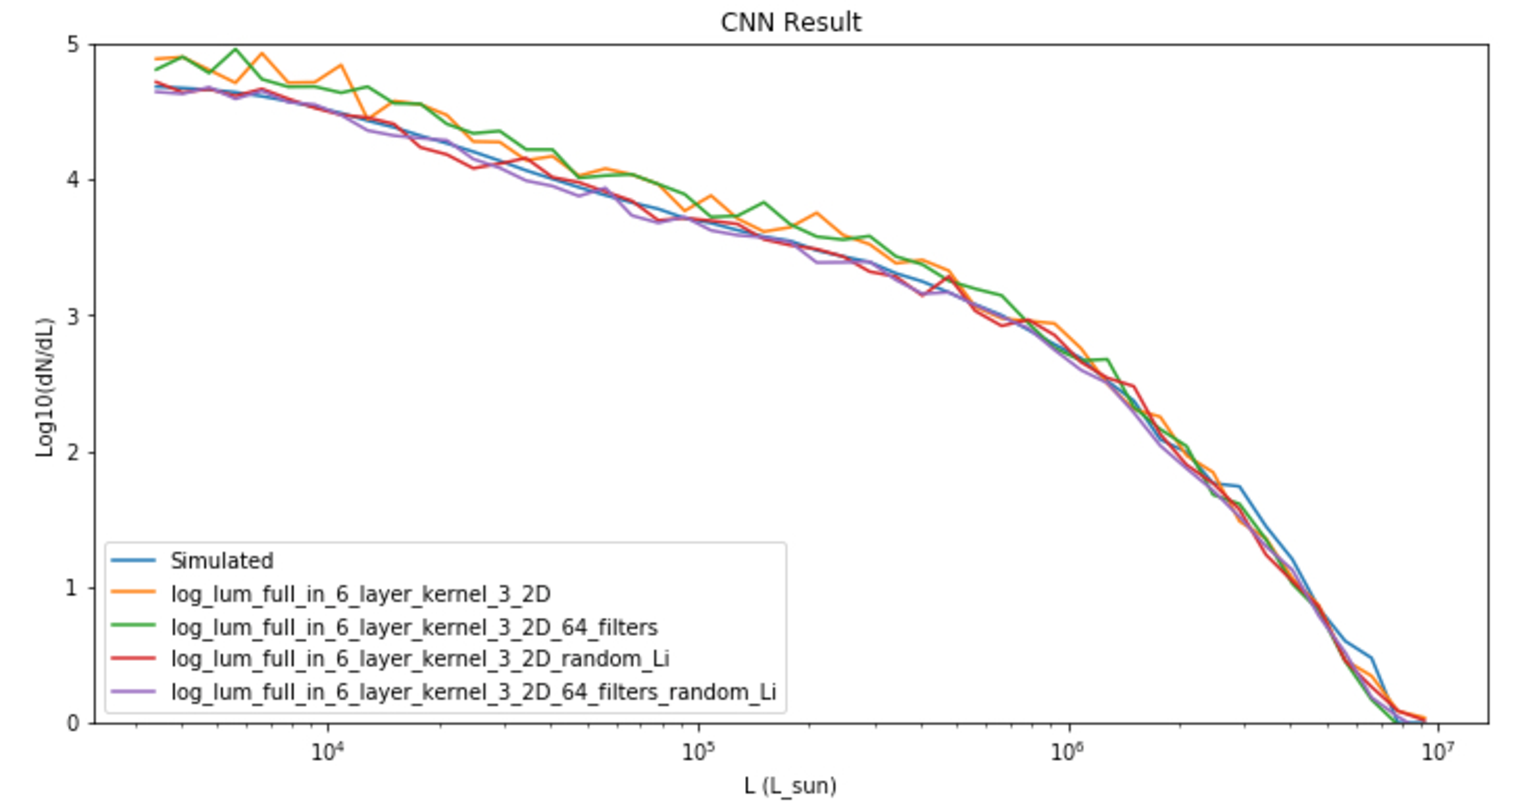
\includegraphics[width=1.0\textwidth]{power_compare_dn.pdf}
			\caption{Output of different CNN architectures for dN.}
			\label{fig:power_compare_dn}
		\end{figure}

		\begin{figure}[H]
			\centering
			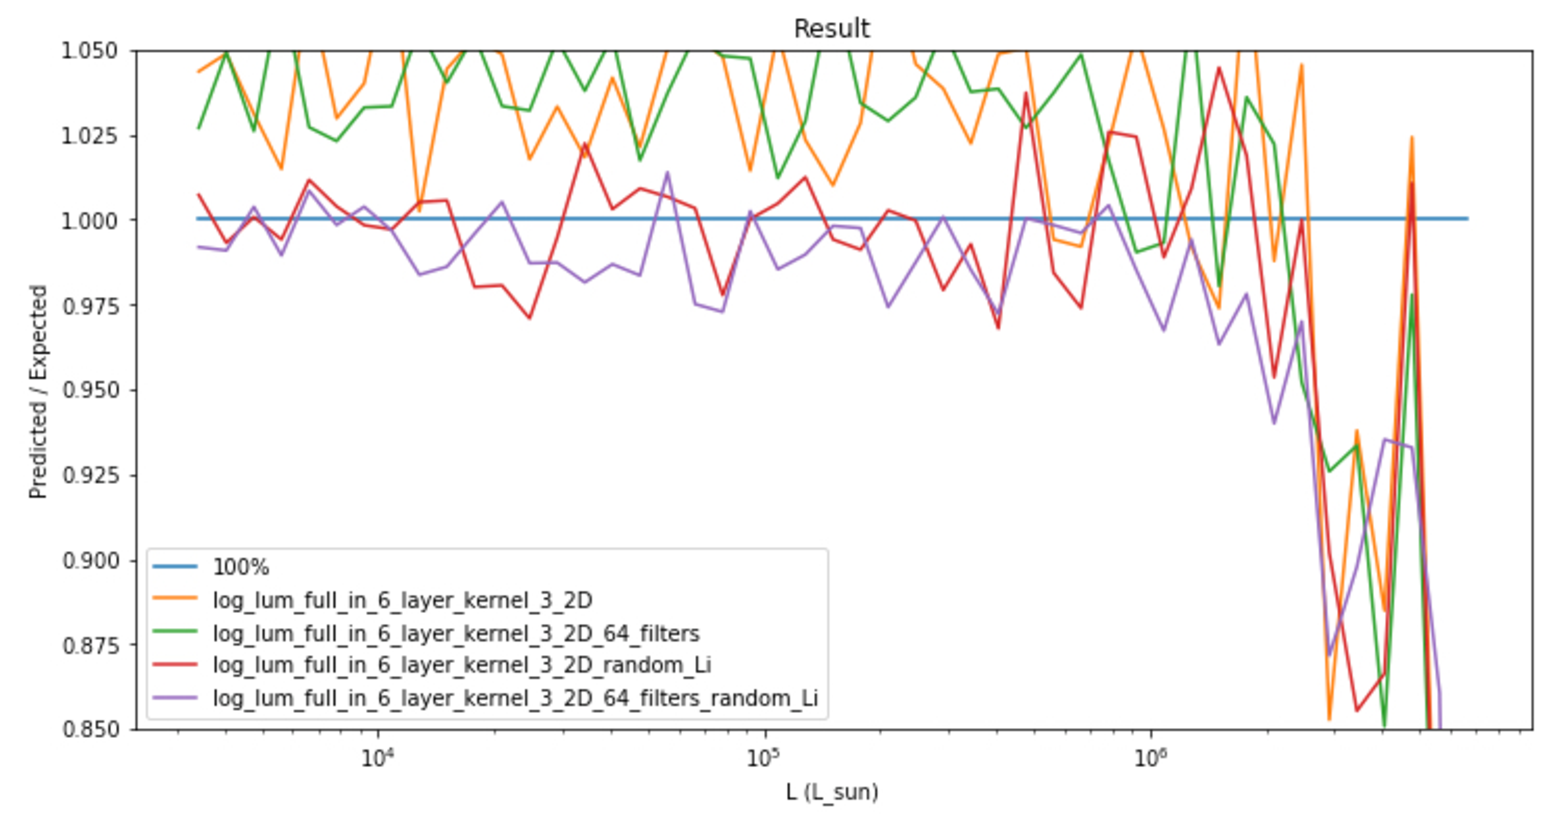
\includegraphics[width=1.0\textwidth]{power_compare_dn_ratio.pdf}
			\caption{Same as \cref{fig:power_compare_dn}, but showing ratio of CNN output to underlying value instead of raw values.}
			\label{fig:power_compare_dn_ratio}
		\end{figure}

		\begin{figure}[H]
			\centering
			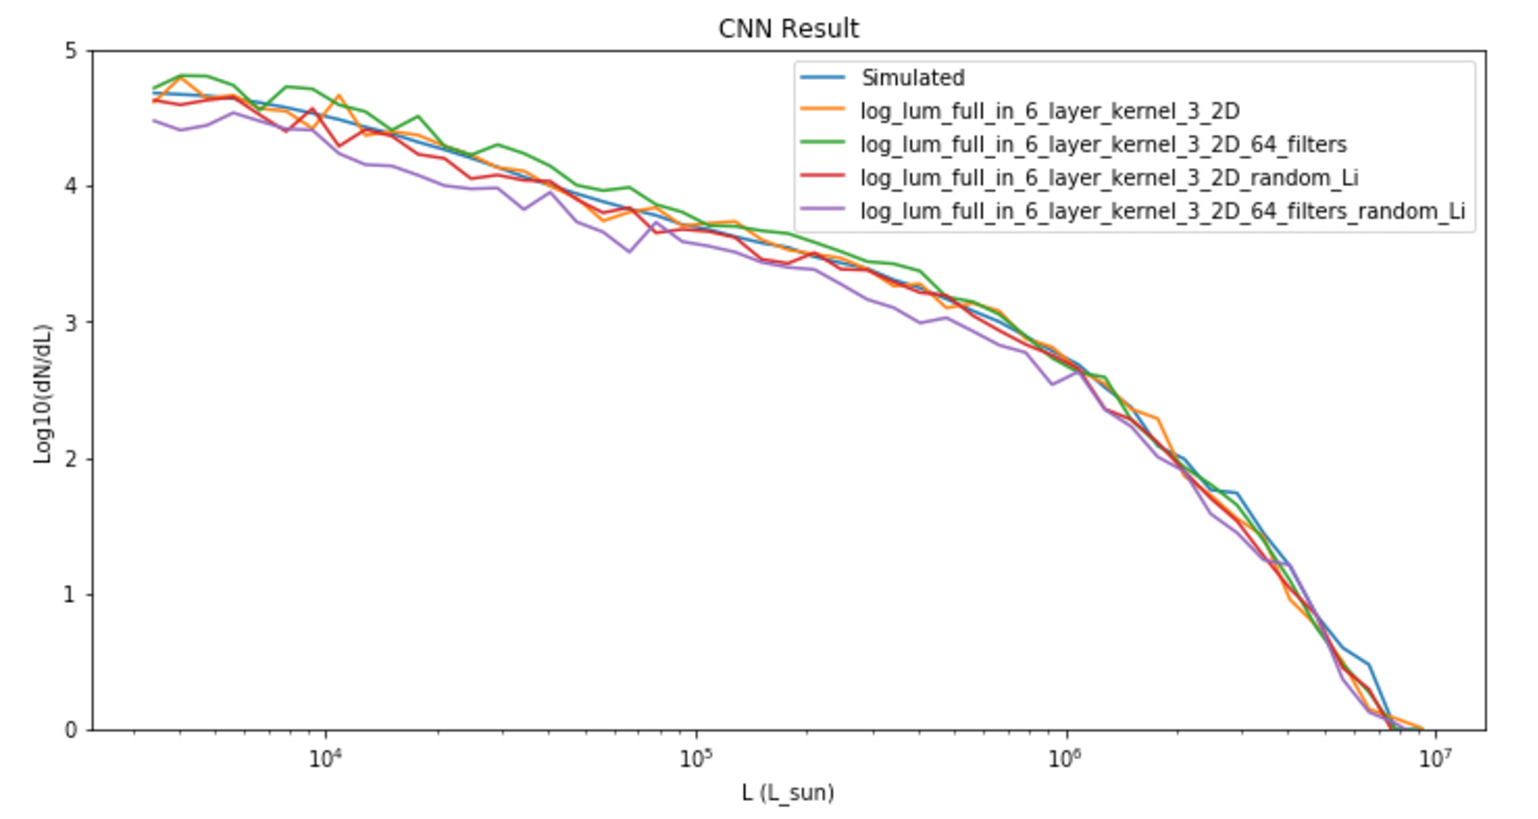
\includegraphics[width=1.0\textwidth]{power_compare_noise_dn.pdf}
			\caption{Output of different CNN architectures for dN with 11 \(\mu K\) white noise.}
			\label{fig:power_compare_noise_dn}
		\end{figure}

		\begin{figure}[H]
			\centering
			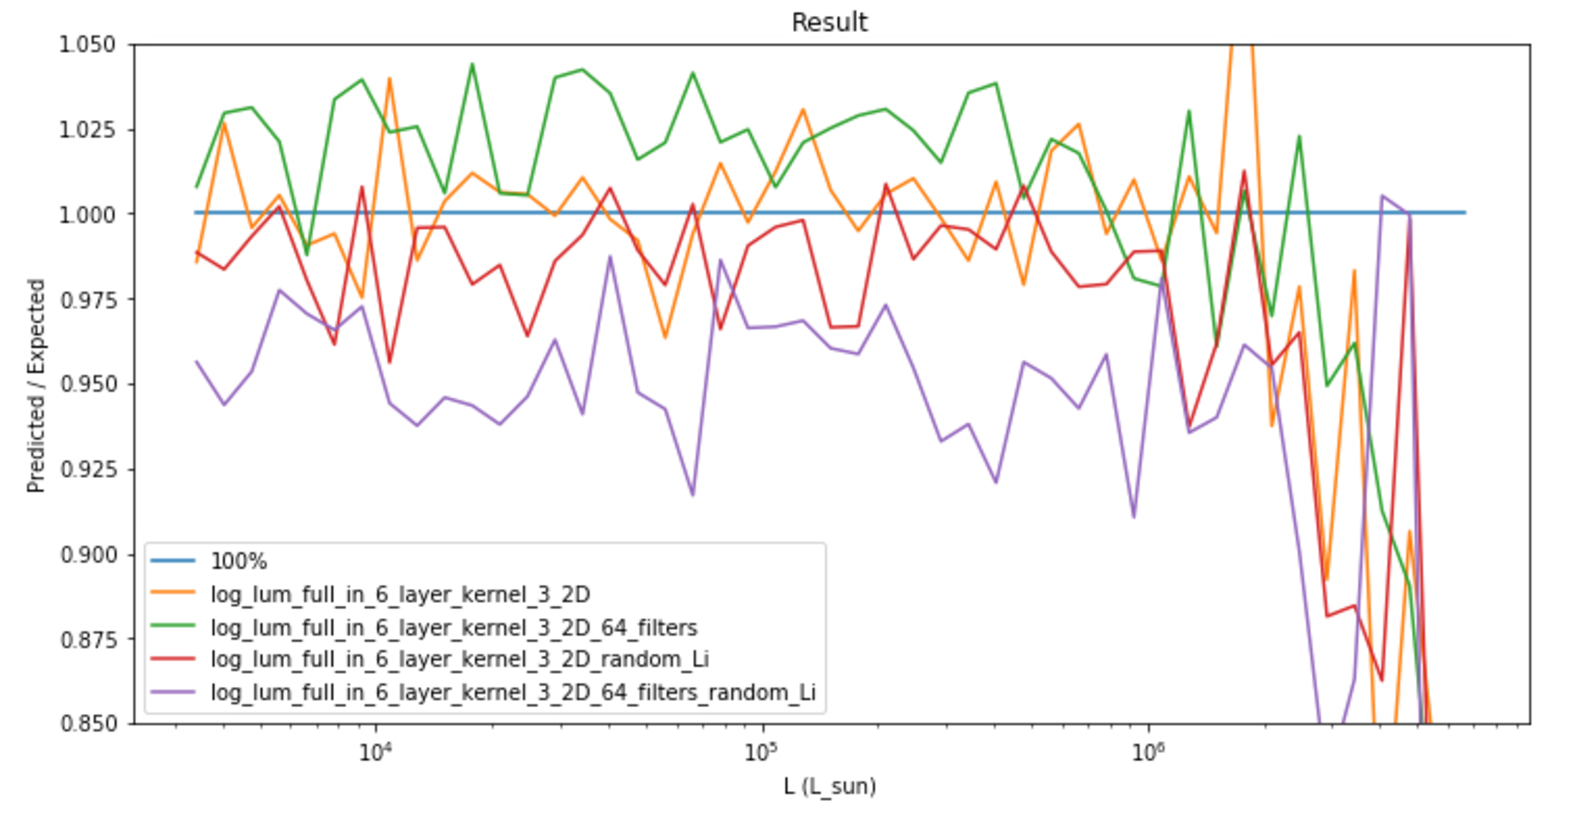
\includegraphics[width=1.0\textwidth]{power_compare_noise_dn_ratio.pdf}
			\caption{Same as \cref{fig:power_compare_noise_dn}, but showing ratio of CNN output to underlying value instead of raw values.}
			\label{fig:power_compare_noise_dn_ratio}
		\end{figure}

		In \cref{fig:log_lum_full_in_6_layer_kernel_3_2D_history_2,fig:log_lum_full_in_6_layer_kernel_3_2D_64_filters_history_2,fig:log_lum_full_in_6_layer_kernel_3_2D_random_Li_history,fig:log_lum_full_in_6_layer_kernel_3_2D_64_filters_random_Li_history} we see the training history for the models being looked at in this section.  For the non-noisy models the plot is messed up.  Epochs 100-175 for them are from a different run.  Do to how I programmed things and the fact that I used the same names it did something stupid.  Those epochs are an artifact and did not affect how the models trained this time.  It only had 200 epochs of training and I didn't feel like trying to fix the plots and make them better.

		\begin{figure}[H]
			\centering
			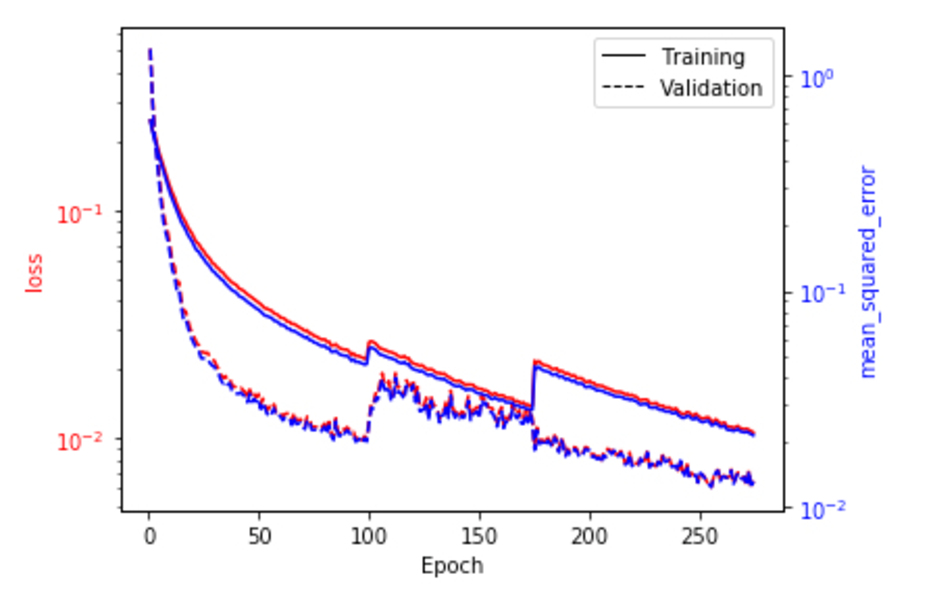
\includegraphics[width=0.8\textwidth]{log_lum_full_in_6_layer_kernel_3_2D_history_2.pdf}
			\caption{Loss history of the training of the log\_lum\_full\_in\_6\_layer\_kernel\_3\_2D model.  See the above paragraph about epochs 100-175.}
			\label{fig:log_lum_full_in_6_layer_kernel_3_2D_history_2}
		\end{figure}

		\begin{figure}[H]
			\centering
			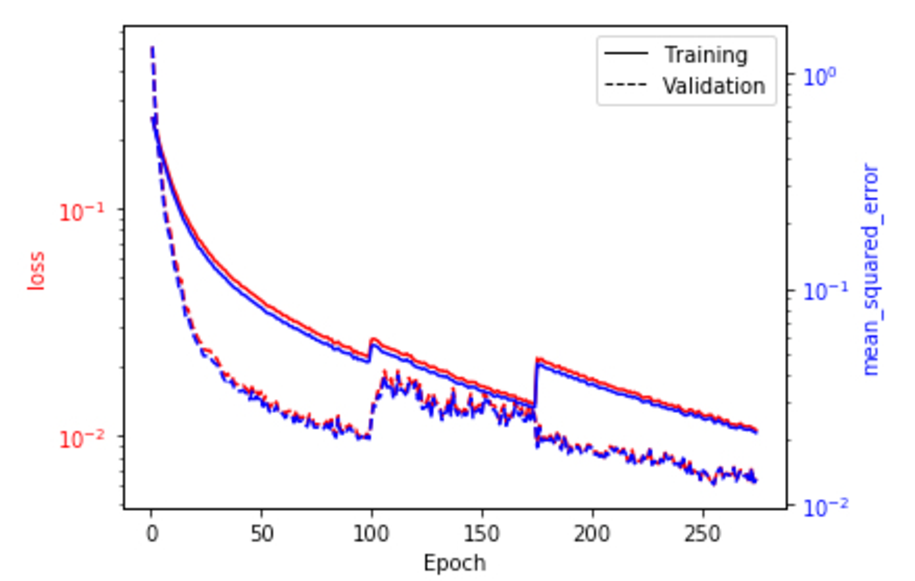
\includegraphics[width=0.8\textwidth]{log_lum_full_in_6_layer_kernel_3_2D_64_filters_history_2.pdf}
			\caption{Loss history of the training of the log\_lum\_full\_in\_6\_layer\_kernel\_3\_2D\_64\_filters model.  See the above paragraph about epochs 100-175.}
			\label{fig:log_lum_full_in_6_layer_kernel_3_2D_64_filters_history_2}
		\end{figure}

		\begin{figure}[H]
			\centering
			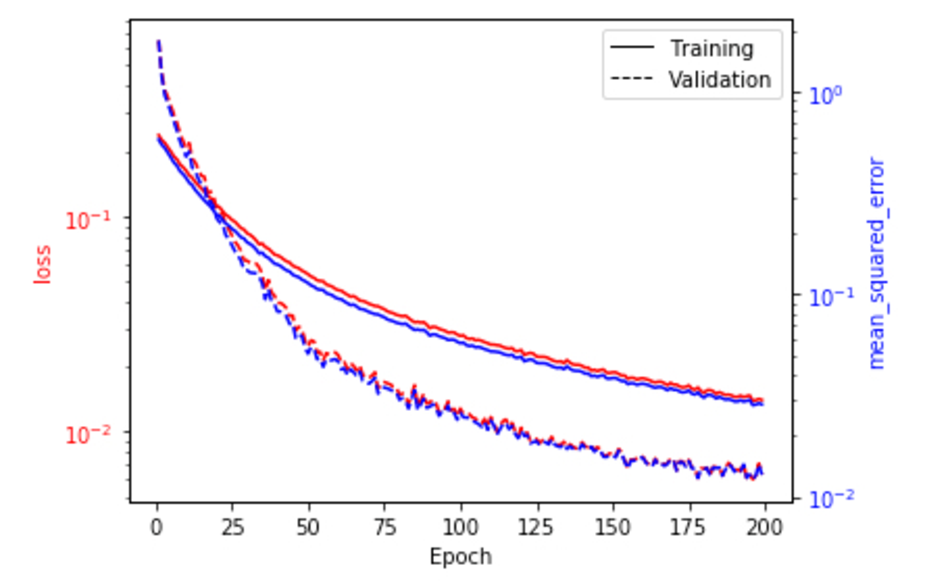
\includegraphics[width=0.8\textwidth]{log_lum_full_in_6_layer_kernel_3_2D_random_Li_history.pdf}
			\caption{Loss history of the training of the log\_lum\_full\_in\_6\_layer\_kernel\_3\_2D\_random\_Li model.}
			\label{fig:log_lum_full_in_6_layer_kernel_3_2D_random_Li_history}
		\end{figure}

		\begin{figure}[H]
			\centering
			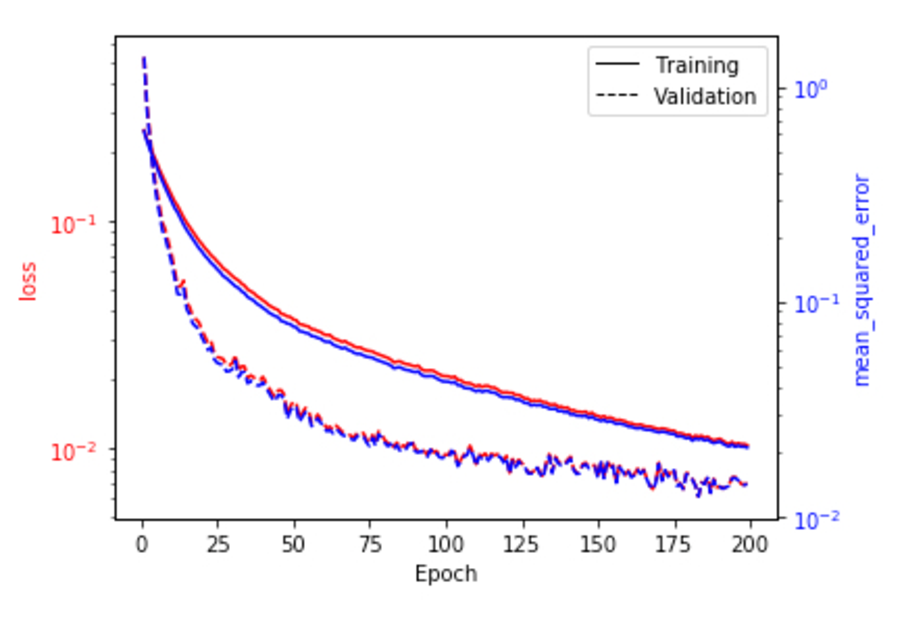
\includegraphics[width=0.8\textwidth]{log_lum_full_in_6_layer_kernel_3_2D_64_filters_random_Li_history.pdf}
			\caption{Loss history of the training of the log\_lum\_full\_in\_6\_layer\_kernel\_3\_2D\_64\_filters\_random\_Li model.}
			\label{fig:log_lum_full_in_6_layer_kernel_3_2D_64_filters_random_Li_history}
		\end{figure}

		Looking at this it seems like 11 \(\mu K\) of noise doesn't do much to these models, but training on it does help a bit.  Increasing the amount of noise by a factor of 3 does impact things though.  \dnp{I should remember to put in a figure for this}.

		At some point we should actually compare to the power spectrum and and temperature bin method of determining the underlying luminosity function.  Figure \ref{fig:comap_power_spectrum} is the money plot from arxiv:1808.07487 which shows how accurate the power spectrum method is.  One of the issues with this is that the luminosity function being used in the power spectrum paper is a density rather then the raw number count being used in this work so far.  If we were working with real valued data instead of log data this wouldn't be an issue because a ratio gets rid of scaling, but that is not true in log space.

		\begin{equation}
			\frac{x \times a}{y \times a} = \frac{x}{y}
		\end{equation}
		\begin{equation} \label{eq:logs}
			\frac{\log (x \times a)}{\log (y \times a)} = \frac{\log x + \log a}{\log y + \log a} \neq \frac{\log x}{\log y}
		\end{equation}

		This means that converting from a density to number counts or vice versa will change the expected accuracy of the technique.  Figure \ref{fig:lum_func_size} shows the magnitude of a random map from the CNN training.  It has values that are more then 6 orders of magnitude greater then the ones used in the power spectrum method.  In Eq. \eqref{eq:logs} this would equate to having \(a = 10^6\).  The \(\log a\) terms will dominate in some regions of the ratio compared to the \(\log x\) and \(\log y\) terms.  The \(\log x\) and \(\log y\) terms represent the CNN prediction for the luminosity function and the underlying value and in density space will have values between -1 and -6.

		\begin{figure}[H]
			\centering
			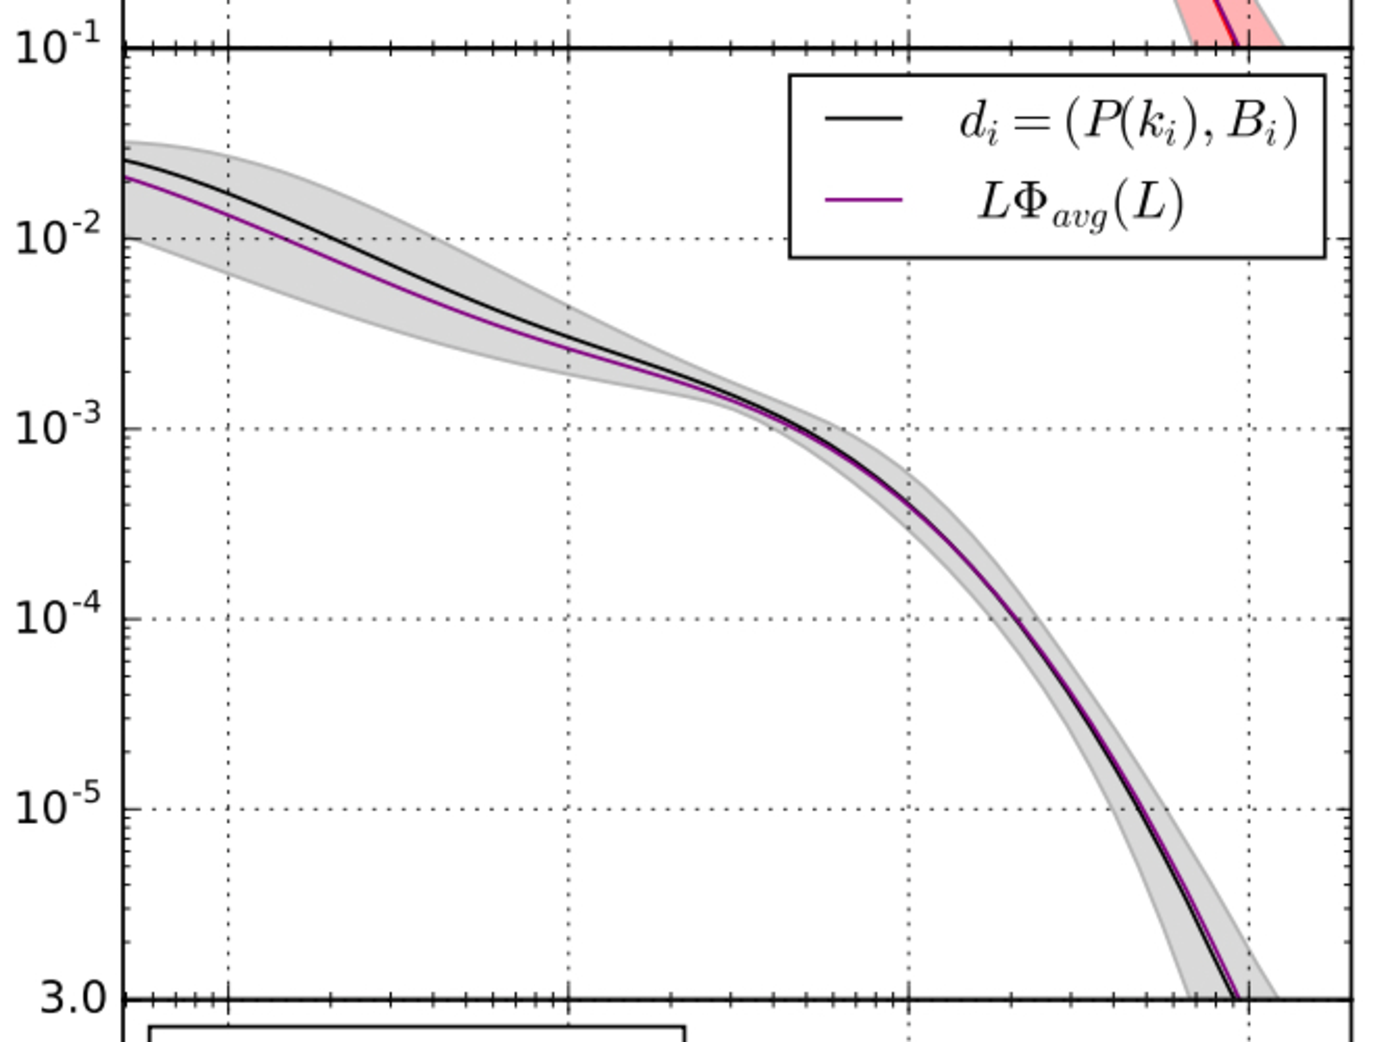
\includegraphics[width=0.9\textwidth]{comap_power_spectrum.pdf}
			\caption{Figure from arxiv:1808.07487 showing the accuracy of the power spectrum luminosity function prediction technique.  The y-axis is a luminosity function density instead of raw number count and the x-axis is just luminosity with the first major tick being \(10^4 L_{sun}\).  The grey shaded region is the 95\% credibility interval of the power spectrum method while the purple line is the underlying luminosity function.}
			\label{fig:comap_power_spectrum}
		\end{figure}

		\begin{figure}[H]
			\centering
			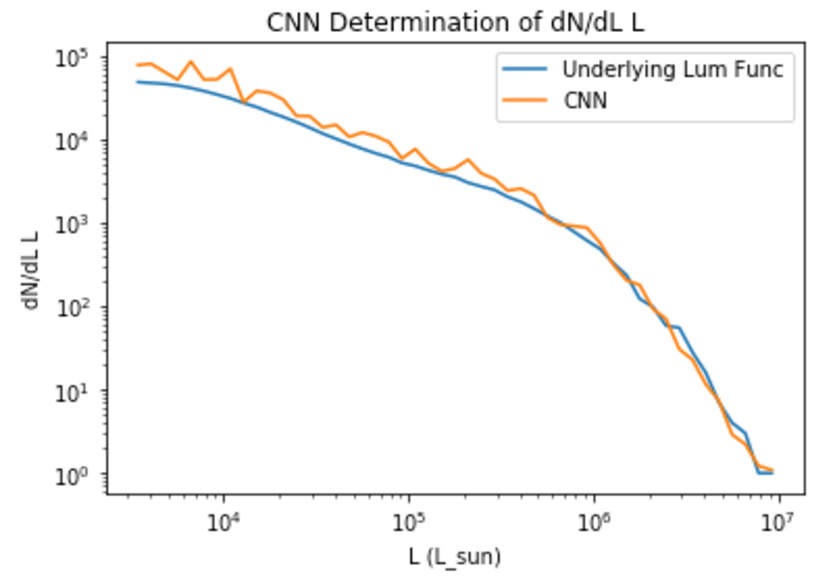
\includegraphics[width=0.9\textwidth]{lum_func_size.pdf}
			\caption{Figure showing the magnitude of luminosity functions used while training the CNNs.  Notice that the y-axis if \cref{fig:comap_power_spectrum} is about 6 orders of magnitude smaller.}
			\label{fig:lum_func_size}
		\end{figure}

		We must also figure out how to display our results in a statistical manor like that of the ones shown in \cref{fig:comap_power_spectrum}.  To do this we need the variance (with respect to the underlying luminosity function) of our CNN models.  To calculate this I run a model on 40 different maps.  For each luminosity I calculate the variance of the CNN luminosity functions with respect to the underlying function.  From this I then calculate the standard deviation (std) and can get the 95\% confidence interval using twice the std.  When comparing the accuracy of the CNN by eye before I never thought about the 95\% confidence interval used in the power spectrum paper so it really doubles the inaccuracy I was observing.  \cref{fig:no_noise_compare,fig:noise_compare} show the results for this with and without noise as well as the confidence interval for the power spectrum method.  We can see that the CNN method is not as good as we believed.  When comparing the correct things the CNN method is not the clear better choice.  It is better at lower luminosities up until around \(few \times 10^5\) and stays worse until around \(10^6\) where the two methods are roughly comparable again.

		At a glance both methods seem comparable.  Further in there are some differences.  The CNN method is slow to train, but fast to get a luminosity function from a given map after training.  I'm not sure about the speed of the power spectrum method.  Running an MCMC is not usually the fastest thing around.  The power spectrum method also takes into account a prediction of the underlying luminosity function.  A different underlying function then the predicted one would probably cause issues.  The CNN needs to train on simulated maps, so using maps made from multiple models will reduce accuracy, but I believe it shouldn't be as bad as with the power spectrum.  \dnp{This should be tested later.}  \dnp{It hasn't been better, but the CNN might be better with foregrounds.  This really needs to be tested.}  

		\begin{figure}[H]
			\centering
			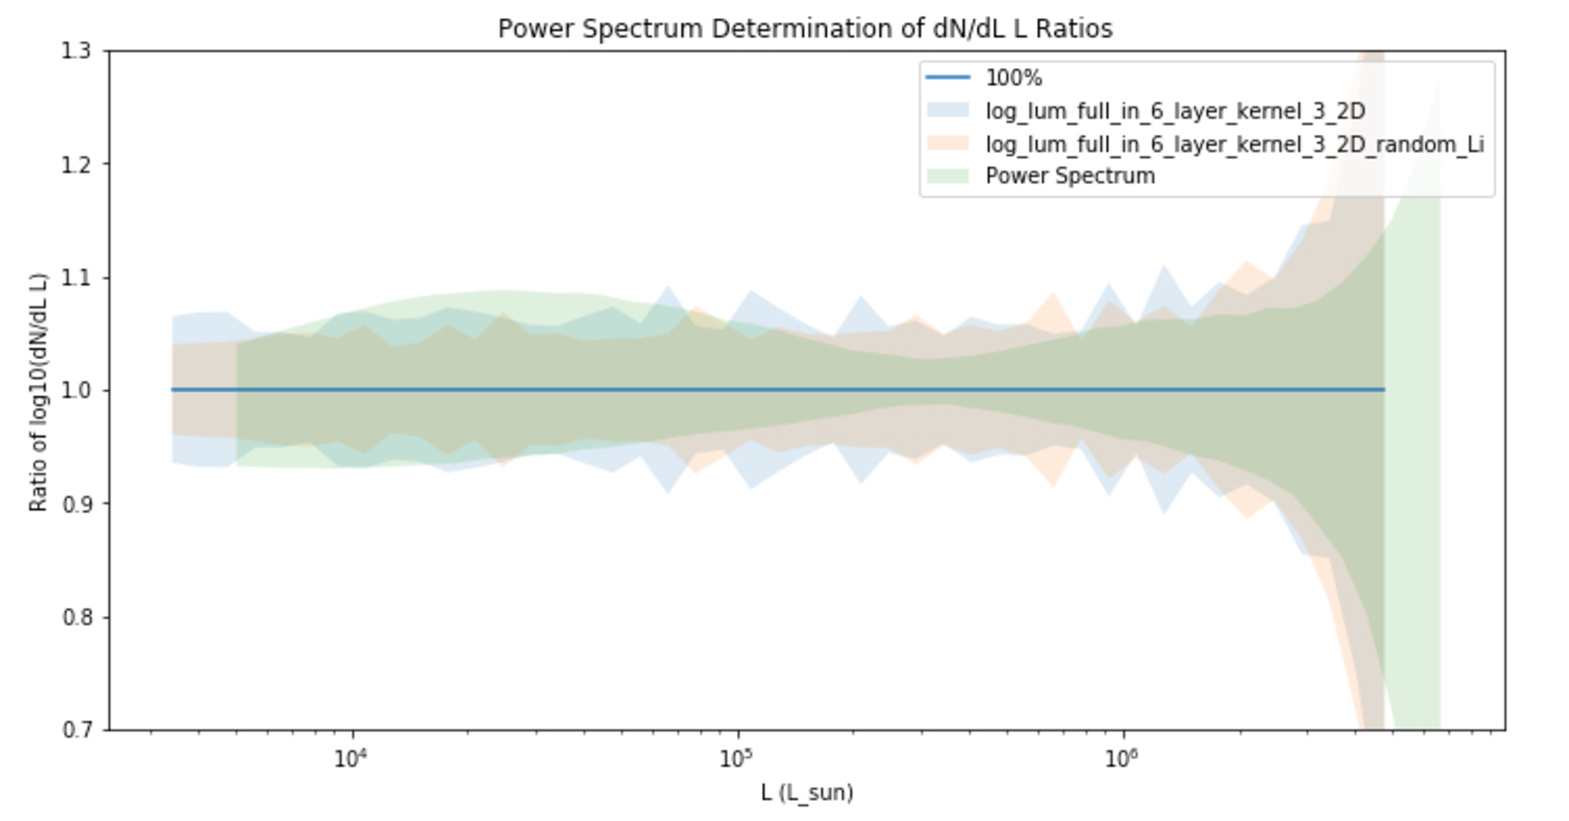
\includegraphics[width=1.1\textwidth]{no_noise_compare.pdf}
			\caption{Comparison of different methods to determine the underlying luminosity function of an intensity map.  The shaded regions are the 95\% credibility interval or the 2 \(\sigma\) error bounds.}
			\label{fig:no_noise_compare}
		\end{figure}

		\begin{figure}[H]
			\centering
			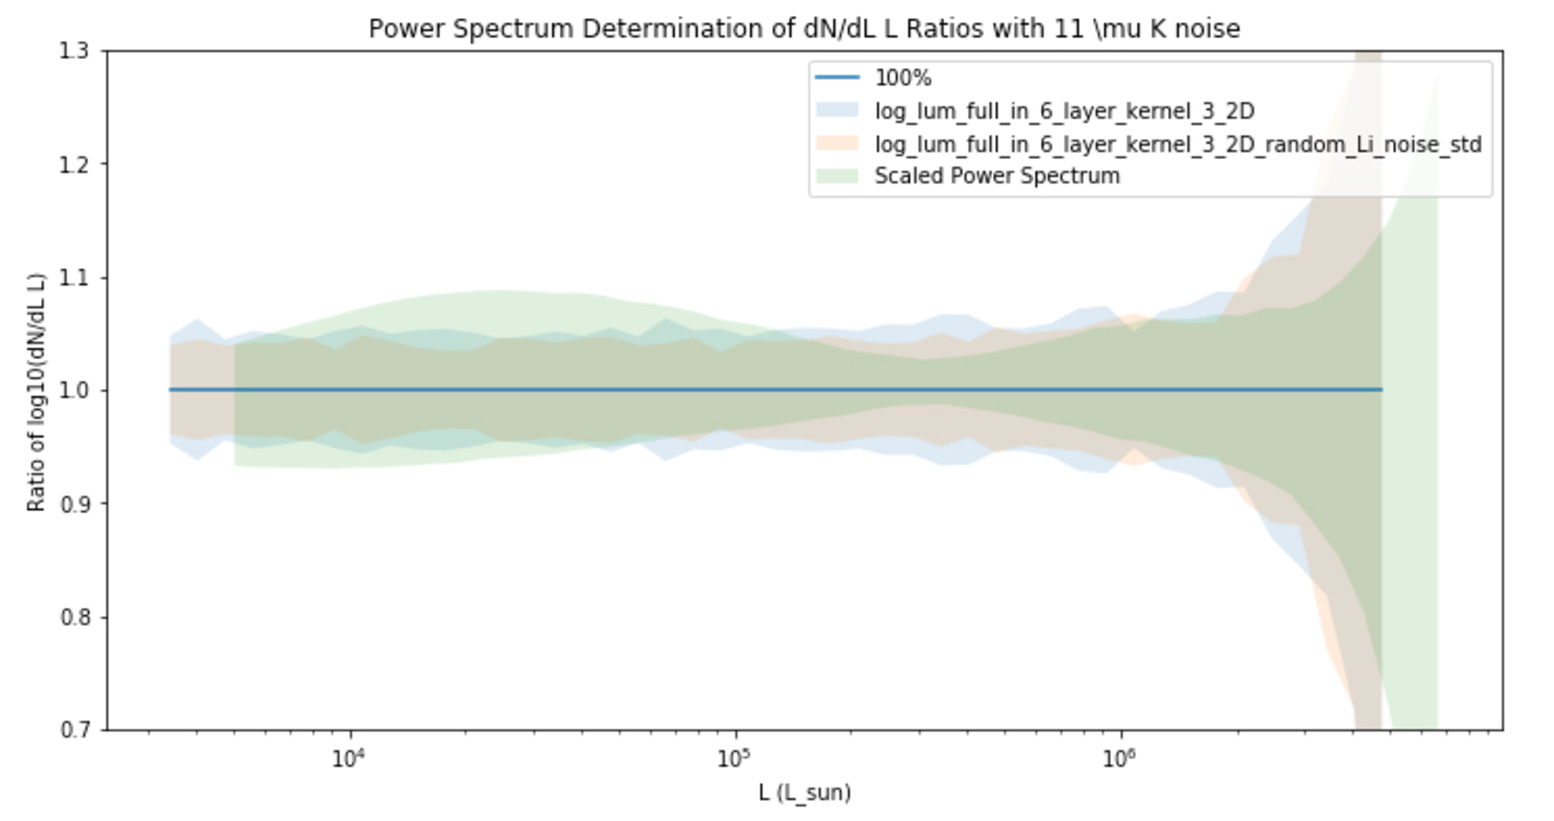
\includegraphics[width=1.1\textwidth]{noise_compare.pdf}
			\caption{Same as \cref{fig:no_noise_compare}, but with 11 \(\mu K\) white noise.}
			\label{fig:noise_compare}
		\end{figure}

	\section{Accidentally Memorizing} \label{sec:mem}
		After training a model on the Li et al model we wanted to test how good it could do with an intensity map produced with another underlying model.  \cref{fig:Li_Model_with_Padmanabhan} shows the result of that and it is not good.  It appears that the CNN memorized the basic structure of the Li model rather then learning anything.  Because of this we need(ed) to do more testing.  

		\begin{figure}[H]
			\centering
			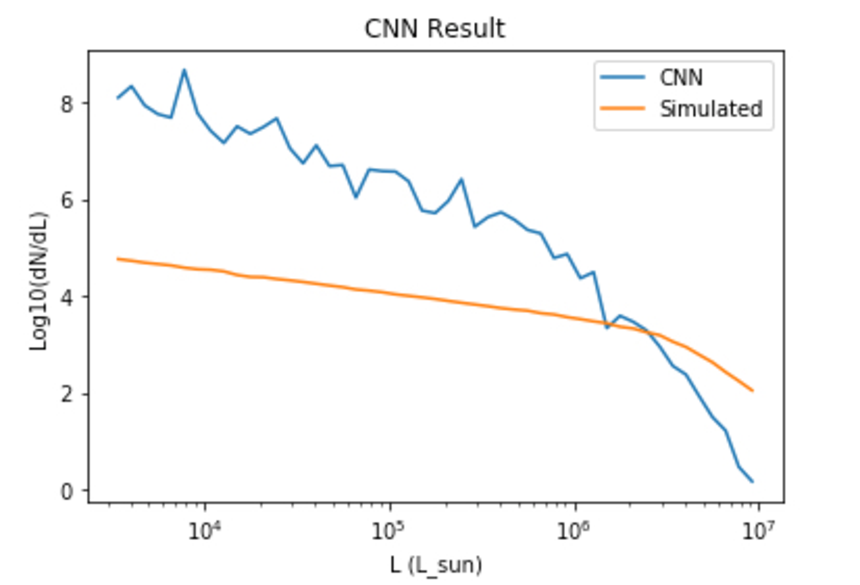
\includegraphics[width=0.8\textwidth]{Li_Model_with_Padmanabhan.pdf}
			\caption{The prediction of a CNN trained on Li models when tested on an intensity map produced by a Padmanabhan model.}
			\label{fig:Li_Model_with_Padmanabhan}
		\end{figure}

	\section{Using Random Parameters in Models} \label{sec:rand}
		Because of the memorization that happened in \cref{sec:mem} we needed to train a model on more then data produced with the base parameters for a model.  Each model we use has parameters in them that must be set to convert the halo catalog into a number of halos that then get converted to an intensity map.  Originally we were testing on maps made using the Li model but with the best fit parameters.  By changing these parameters we would change the number of halos expected to be in each map.  This change in number of halos will lead to different intensity maps.

		Intensity maps were made using a different realization of the Li model for each map with a random draw of what the needed parameter values would be.  These maps were then used to a train a CNN and it was a failure.  It had no predictive powers.  The reason why can be seen in \cref{fig:variation_in_Li}.  The range of different luminosity functions produced is huge.  There is too much to try and learn.  It is not learning variations of a general pattern or two, it is trying to learn many completely different things.  A simple model should not be able to learn this.

		\begin{figure}[H]
			\centering
			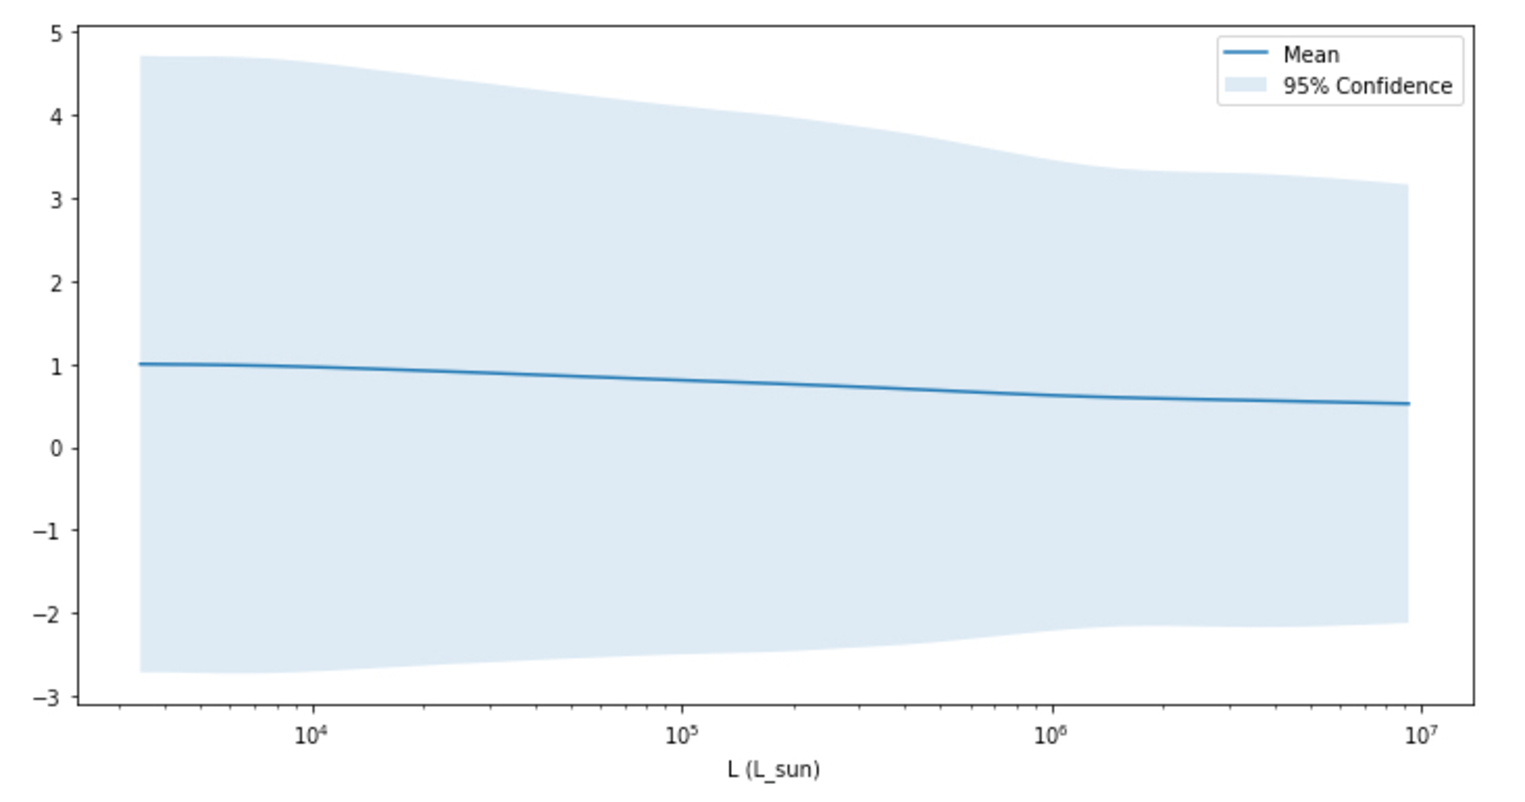
\includegraphics[width=1.0\textwidth]{variation_in_Li.pdf}
			\caption{The solid line is the ratio of the mean luminosity function for 1000 realizations of Li intensity maps to the value of the mean at the lowest luminosity value.  The filled in region is related to the 2 \(\sigma\) region.  The limits are just mean \(\pm 2 \sigma\) where \(\sigma\) is calculated for each luminosity \(L\).  The upper limit is correct, but the bottom one doesn't really mean anything.}
			\label{fig:variation_in_Li}
		\end{figure}

		If instead we were to look at the variation produced when using the default values we would get \cref{fig:variation_in_default_Li}.  The variation is much smaller.  If instead we look at \cref{fig:variation_in_default_Li_local} we see the variation is around 5-10\% for the most part.  Now comparing to \cref{fig:noise_compare} we see variation of the 6 layer model is actually slightly less then the 5-10\% expected by looking at different views of the catalog that produces the intensity maps.  This means the CNN is learning something more then just the basic shape of the default values.  If it didn't, it would have variation on the same order.  \dnp{This seems good!}

		\begin{figure}[H]
			\centering
			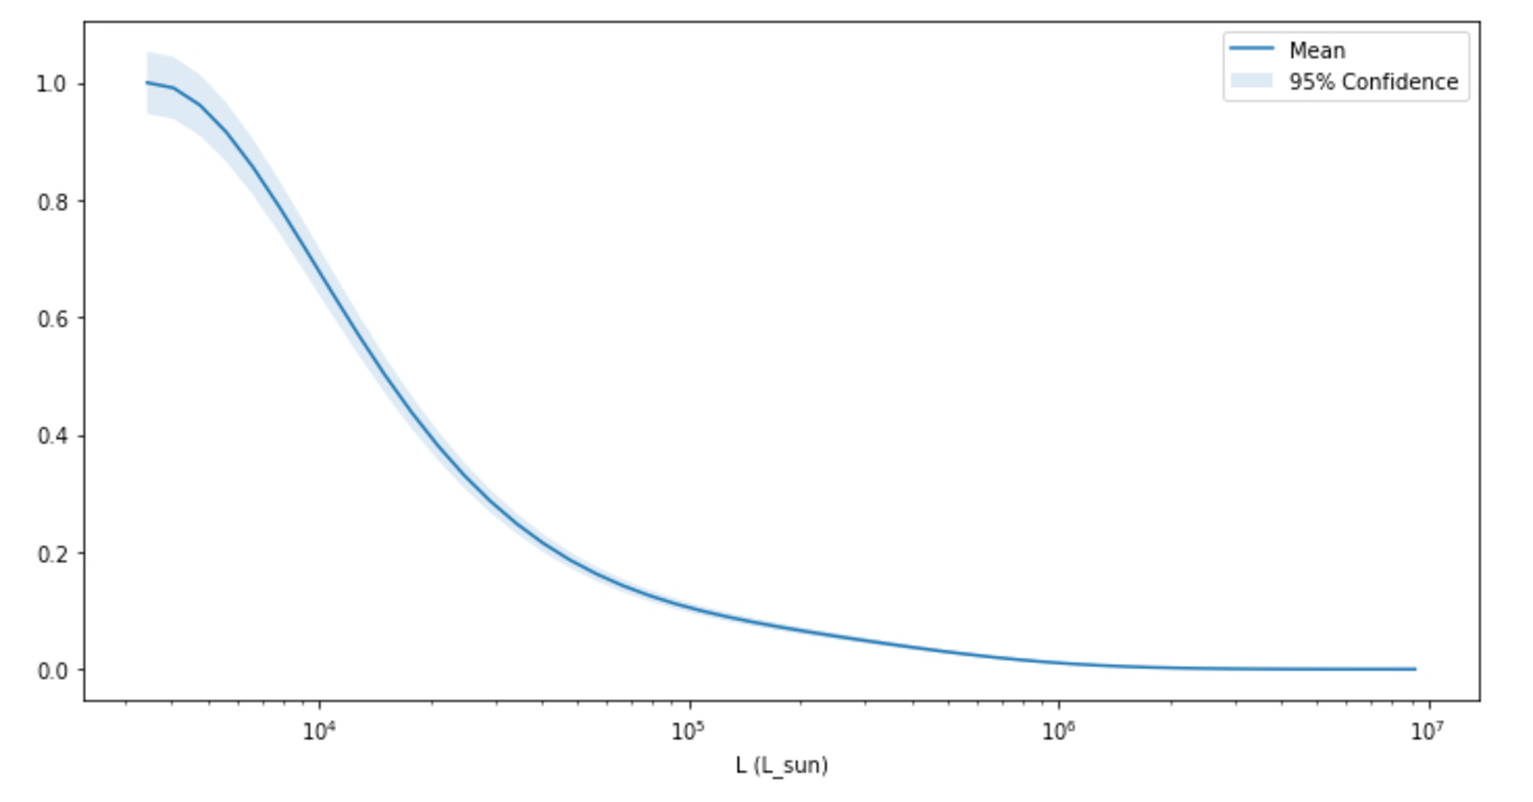
\includegraphics[width=1.0\textwidth]{variation_in_default_Li.pdf}
			\caption{Same as \cref{fig:variation_in_Li}, but when only using the default parameters in the Li model when producing intensity maps.}
			\label{fig:variation_in_default_Li}
		\end{figure}

		\begin{figure}[H]
			\centering
			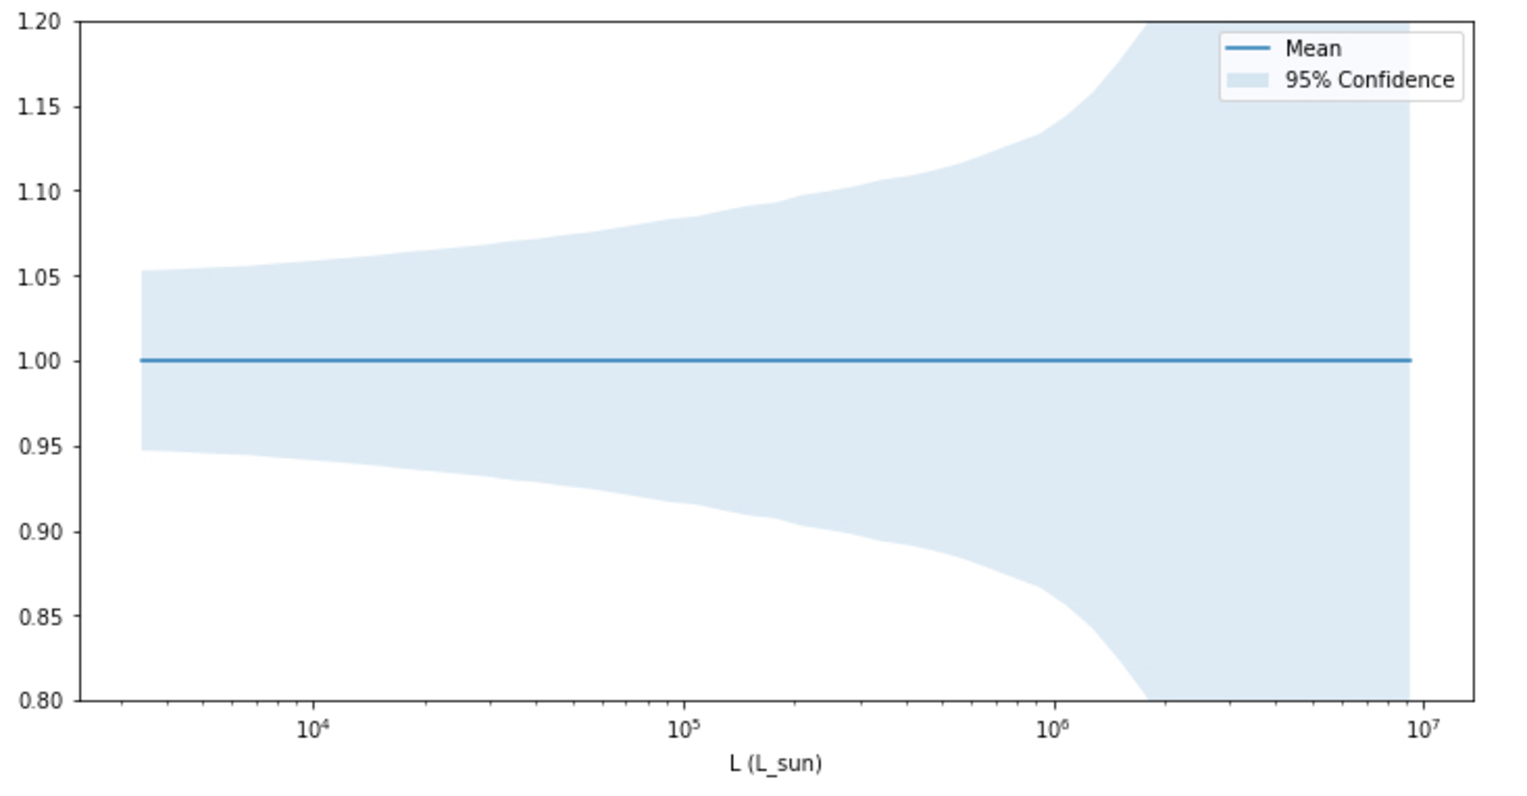
\includegraphics[width=1.0\textwidth]{variation_in_default_Li_local.pdf}
			\caption{Similar to \cref{fig:variation_in_default_Li}, but instead of get the ratio with respect to the value of the mean at the lowest luminosity, finds the ratio with respect to the mean at every luminosity.  This allows us to see variations relative to the mean at each luminosity.}
			\label{fig:variation_in_default_Li_local}
		\end{figure}

	\section{Comparing Multiple Models} \label{sec:mult}
		Besides testing with random draws of parameter models we also tested using multiple models at once.  The models tested where the Li, Padmanabhan and Breysse (power law) models and used the default parameters.  As was par for the course, this failed as well and can be seen in \cref{fig:multi_model_Padmanabhan,fig:multi_model_Li,fig:multi_model_Breysse}.  These figures are representative of their respective models.  I believe the reason for this is due to the power law model not extending far enough down to low intensities.  This drop at lower luminosity to the zero sources is a much different feature then anything and in my opinion is probably what makes this not work out well.  \dnp{I have no proof of that at the moment.}  That being said, this does seem to work as a classifier.  The prediction for each model is different for each model.  I don't know how much work it would be, but I think this trained CNN could be used to jump start the training of a classifier with similar architecture.  The final layer of the current CNN would need to be replaced with 3 neurons instead of 50 where each neuron represents a model instead of a value of the luminosity function.  \dnp{Maybe try to do this without Breysse model.}

		\begin{figure}[H]
			\centering
			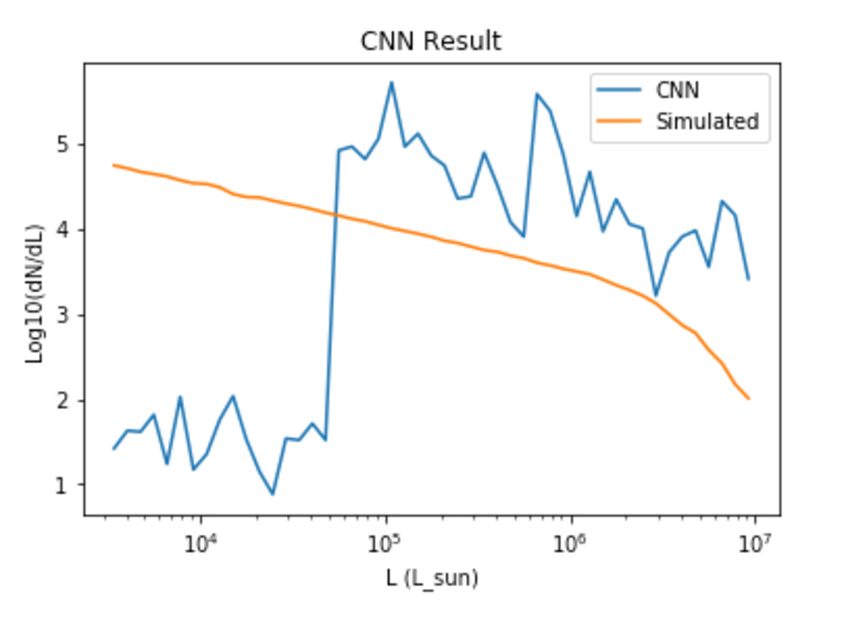
\includegraphics[width=0.9\textwidth]{multi_model_Padmanabhan.pdf}
			\caption{Multi model CNN trying to predict the luminosity function from an underlying Padmanabhan model.  The CNN was trained on Li, Padmanabhan and Breysse models.}
			\label{fig:multi_model_Padmanabhan}
		\end{figure}

		\begin{figure}[H]
			\centering
			\includegraphics[width=0.9\textwidth]{multi_model_Li.pdf}
			\caption{Same as \cref{fig:multi_model_Padmanabhan} but with an underlying Li model.}
			\label{fig:multi_model_Li}
		\end{figure}

		\begin{figure}[H]
			\centering
			\includegraphics[width=0.9\textwidth]{multi_model_Breysse.pdf}
			\caption{Same as \cref{fig:multi_model_Padmanabhan} but with an underlying Breysse model.}
			\label{fig:multi_model_Breysse}
		\end{figure}

	\section{Memorization Realization} \label{sec:ohcrap}

		For the past couple weeks I have been trying to get a CNN to predict the luminosity function from maps made with a single model, but varying parameters as seen in \cref{sec:rand}.  The point is to learn how to actually read the map and learn to count the number of sources directly from it.  I have no come to the full realization that we have so far not done anything like that.  What has been happening is that the network learns the least offensive luminosity function and more or less just sticks with that.  Least offensive here is meaning that this is the default luminosity function that will minimize loss for the entire dataset without any change.  It then tries to learn small perturbations on top of it.  This works for a single realization of an underlying model because the changes to the expected luminosity function in a given map are very small.  This does not work when you vary underlying model parameters.

		I've been trying many different models to learn to read maps made with varying parameters, but nothing has worked so far.  I've tried 2D and 3D basic models and a resnet model.  I've tried with more layers and filters as well as lowering the learning and tweaking hyper parameters.  The same thing happens for all of them, the training loss data reaches a constant value (around 0.1 - 0.3) and stays there for the entire training process.  The validation loss data just fluctuates.  An example of this is seen in \cref{fig:failed_learning}.  The output luminosity function barely changes between maps.

		\begin{figure}[H]
			\centering
			\includegraphics[width=0.9\textwidth]{failed_learning.pdf}
			\caption{Training and validation loss and metrics for the training of a resnet CNN.  It should be clear that the training data didn't learn anything.  It memorized something at the very beginning and stuck with it.  The network was trained on maps made with small variation of parameters in the Li model.}
			\label{fig:failed_learning}
		\end{figure}

		The failure of the models to learn anything can be seen in \cref{fig:no_intensity}.  The input that led to this luminosity function was actually a blank map.  Every value in it was set to 0.  We see that the CNN just ignored the input for the most part and just always made the same luminosity function with tiny changes on it.

		\begin{figure}[H]
			\centering
			\includegraphics[width=0.9\textwidth]{no_intensity.pdf}
			\caption{The CNN and smoothed CNN lines here are the result of a CNN given an empty intensity map (every value was 0 in it).  The network was trained on maps made with small variation of parameters in the Li model.  Ignore the green simulated line.}
			\label{fig:no_intensity}
		\end{figure}

		So now we need to figure out how to get around this and do what we wanted to do from the beginning.  We need to just learn how to translate a map directly to the number of sources in a luminosity bin.  One possible issue is that the intensity maps are very sparse.  Around 90\% of pixels have no luminosity in them.  What the CNNs have been doing is more or less ignoring the input and just using the initial biases.  I'm starting to try and shrink the size of the maps before being used.  If instead of 256x256 for each image we used 128x128 or 64x64 we would get 25\% and 50\% of pixels having non-zero values respectively.  With this non-sparse data hopefully the network actually learns rather than memorizes.

		Making the maps smaller didn't help... \\

		I don't know if it was mentioned in here yet, but instead of working with maps made using an underlying Li luminosity function and the fiducial mean and errors I used one with the fiducial mean, but only 10\% of the fiducial errors.  The idea is that it would lower the expected output parameter space.  This didn't fix things.

		Messing around with what the dropout was and where it was located didn't really help.  I also tried using specific pooling functions instead of convolutions that pool and that didn't really do anything.  One thing that had a minor result is removing the bias value from the first layer.  The idea was that if the weights were small for the first layer and the bias big it could be that the map was ignored and the bias value determining most things.  This seems to be true considering that an empty map gave the same output as a non-empty one.  Removing the bias helped a small amount.  Removing it gave the same general shape, but allowed the amplitude at low luminosity to go up and down some.  It was not a real fix.

		I'm annoyed at how simple the solution was, but whatever, better late then never.  What got things working at the end was switching over to using Adam for the optimizer instead of stochastic gradient descent (SGD).  \dnp{I should make sure I fully understand Adam at some point.}

	\section{Something Finally works} \label{sec:works}
		After switching over to Adam I got a run to work.  I first tried to train on only 12 maps and make sure it could over-fit, which it did, then I moved on to 500 maps.  The results with 500 maps was wonderful.  It's fitting the entire dataset really well after 100 epochs.

		The network that is currently working is as follows
		\begin{itemize}
			\item 6 layers.  Each layer is a convolution with batch normalization, dropout and then another convolution that acts as a pooling layer.
			\item 2 dense layers at the end.  The first has 1000 neurons and the second and last layer of the network has 49, one for each output.
			\item 64 filters on the first convolutional layer and doubling every layer.
			\item 50\% dropout
			\item 0-padded sides
			\item 3d convolutions with kernel size 3
			\item Pooling done with 3d convolutions with kernel size 2 and stride 2
		\end{itemize}

		The data the network trained on was as follows
		\begin{itemize}
			\item Maps are pre-pooled.  Instead of being 256X256X100 I am using 64X64X10 maps.  I pool by converting 4X4X10 regions into a single pixel with the intensity being the sum of all of the previous individual ones.
			\item The output luminosity function is log valued
			\item The input map is given an extra intensity of 1e-6 for each pixel and then log valued.  The extra 1e-6 intensity prevents taking the log of 0.  Finally every pixel in the log map gets an extra 6 added to it so that pixels with no intensity would have 0 intensity in whatever new units we have. 
			\item I used only 500 maps for training data.  I was starting with a low number (12) to make sure overfitting could happen.  It did then I was going to slowly increase up to 80\% of the total number of maps (<6000 maps at the moment), but using only 500 maps worked really well.
			\item The maps being used were done using a Li model for the underlying luminosity function with the fiducial mean, but errors that were 10\% of reported ones.  I tried using the full error, but it does not work for this setup.  It hasn’t finished running at the moment, but it’s validation loss is not anywhere near anything good.
			\item Batch size of 40 maps, 100 steps in an epoch (400 maps looked at) and 100 epochs of training.
			\item Validation testing uses 3 steps with the batch size of 40 (120 maps for validation each epoch).
		\end{itemize}

		Figure \ref{fig:adam_good} is of a fairly typical fit of the CNN to a map.  It’s good.  This current CNN when predicting the luminosity function on maps made with different underlying luminosity functions is just as good as our old CNN was for predicting the luminosity function of maps made with the same Li model parameters.  I can tell this because when tested over many maps they give the same training error.  They both gave ~0.006 which doesn’t mean much on it’s own, but you want to minimize that and they both give the same value.  This is good because we are fitting to more complicated data better or just as good as we “fit” to data that was nearly always the same.

		Figure \ref{fig:adam_good_2} shows that the CNN has a little issue when there are not high luminosity objects.  That region is noisy and it likes making smooth curves that don't pick up that noise and the drop to 0 objects perfectly.  It is still good at getting the general tend.  It also can’t handle actual noise yet.  Adding even 1 micro Kelvin messes with the prediction a lot and brings the loss to around 0.5.  Remember that it gives a loss around 0.006 for no noise.

		\begin{figure}[H]
			\centering
			\includegraphics[width=0.9\textwidth]{adam_good.pdf}
			\caption{}
			\label{fig:adam_good}
		\end{figure}

		\begin{figure}[H]
			\centering
			\includegraphics[width=0.9\textwidth]{adam_good_2.pdf}
			\caption{}
			\label{fig:adam_good_2}
		\end{figure}

		Figure \ref{fig:adam_training} shows the training history for the CNN.  For this the loss function was changed to mean\_squared\_error so ``loss'' and ``mean\_squared\_error'' on the plot are the same thing.  The validation data has some large spikes.  This may be due to some maps in the validation data being a decent bit different then the other ones.  This can be investigated later.

		\begin{figure}[H]
			\centering
			\includegraphics[width=0.9\textwidth]{adam_training.pdf}
			\caption{}
			\label{fig:adam_training}
		\end{figure}

	\section{Things to do for Dan in no particular order} \label{sec:todo}
		\begin{enumerate}
			\item \sout{Figure out what a good frequency bin size is}  COMAP can handle around 500 different frequency bins so using 100 is a lower limit.

			\item \sout{Make maps and luminosity functions. Have done this for some maps and have the ability to do this for more.}

			\item \sout{Add in different halo luminosity relations to llm}

			\item \sout{Do some test runs with something basic}

			\item \sout{Make an actual CNN and try training it for an extended period of time}

			\item \sout{Get GPUs working correctly}

			\item \sout{Train on actual luminosity function instead of log(luminosity function). Doesn't give the best results.  See Section \ref{sec:4directValue} (and this was done on \(N\) not \(\phi\)).}

			\item \sout{Get CNN to record loss and metric as it trains}

			\item \sout{Make lots of maps on MARCC to train with.  This will happen soon.}

			\item \sout{Use validation data to see that the model is actually learning and not memorizing.}

			\item \sout{Ability to train on log input data}

			\item \sout{Ability to make noisy maps when producing the maps, or to add noise to maps after the fact}

			\item \sout{See how many filters / layers the gpus can handle for 2D convolutions}

			\item \sout{Figure out what architecture we actually want to use and start the actual training and testing.  Log input or not, \(\phi\) v.s. \(N\), \# of layers, \# of filters.}  6 layers, 32 initial filters, full input, log output, \(dN/dL\) with log spacing of L.  Actually have a ResNet architecture that works well.

			\item Put info in about visualizing layers?  Can do this, but do we care right now?

			\item Foregrounds?

			\item Classifier between models?

			\item More testing around working Adam model.  Expanded maps, train on full data instead of 500 maps, add in noise.
		\end{enumerate}


	
% \bibliography{draft}
\end{document}